%% 
%% Copyright 2007-2020 Elsevier Ltd
%% 
%% This file is part of the 'Elsarticle Bundle'.
%% ---------------------------------------------
%% 
%% It may be distributed under the conditions of the LaTeX Project Public
%% License, either version 1.2 of this license or (at your option) any
%% later version.  The latest version of this license is in
%%    http://www.latex-project.org/lppl.txt
%% and version 1.2 or later is part of all distributions of LaTeX
%% version 1999/12/01 or later.
%% 
%% The list of all files belonging to the 'Elsarticle Bundle' is
%% given in the file `manifest.txt'.
%% 
%% Template article for Elsevier's document class `elsarticle'
%% with harvard style bibliographic references
\documentclass[preprint,12pt]{elsarticle}
\usepackage[justification=centering]{caption}
% updated with editorial comments 8/9/2021
\usepackage{caption}
\usepackage[fleqn]{amsmath}
\usepackage{amssymb}
\usepackage{graphicx}
\usepackage{float}
\usepackage{flushend}
\usepackage{stfloats}
\usepackage{booktabs} %插表格用的宏包
\usepackage{diagbox} %插表格用的宏包
\usepackage{multirow} %插多行表格用的宏包
\bibliographystyle{elsarticle-num}
\biboptions{sort&compress}
\usepackage[utf8]{inputenc}
\usepackage[ruled,vlined]{algorithm2e}
\usepackage{url} % or use 'hyperref' for clickable links
% \usepackage[numbers,sort&compress,square]{natbib}
% \usepackage{amssymb}
% for table
% updated with editorial comments 8/9/2021
%% Use the option review to obtain double line spacing
%% \documentclass[authoryear,preprint,review,12pt]{elsarticle}
%% Use the options 1p,twocolumn; 3p; 3p,twocolumn; 5p; or 5p,twocolumn
%% for a journal layout:
%% \documentclass[final,1p,times,authoryear]{elsarticle}
%% \documentclass[final,1p,times,twocolumn,authoryear]{elsarticle}
%% \documentclass[final,3p,times,authoryear]{elsarticle}
%% \documentclass[final,3p,times,twocolumn,authoryear]{elsarticle}
%% \documentclass[final,5p,times,authoryear]{elsarticle}
%% \documentclass[final,5p,times,twocolumn,authoryear]{elsarticle}
%% For including figures, graphicx.sty has been loaded in
%% elsarticle.cls. If you prefer to use the old commands
%% please give \usepackage{epsfig}
%% The amssymb package provides various useful mathematical symbols
%% The amsthm package provides extended theorem environments
%% \usepackage{amsthm}
%% The lineno packages adds line numbers. Start line numbering with
%% \begin{linenumbers}, end it with \end{linenumbers}. Or switch it on
%% for the whole article with \linenumbers.
%% \usepackage{lineno}
\journal{}

\begin{document}

\begin{frontmatter}

%% Title, authors and addresses

%% use the tnoteref command within \title for footnotes;
%% use the tnotetext command for theassociated footnote;
%% use the fnref command within \author or \affiliation for footnotes;
%% use the fntext command for theassociated footnote;
%% use the corref command within \author for corresponding author footnotes;
%% use the cortext command for theassociated footnote;
%% use the ead command for the email address,
%% and the form \ead[url] for the home page:
%% \title{Title\tnoteref{label1}}
%% \tnotetext[label1]{}
%% \author{Name\corref{cor1}\fnref{label2}}
%% \ead{email address}
%% \ead[url]{home page}
%% \fntext[label2]{}
%% \cortext[cor1]{}
%% \affiliation{organization={},
%%            addressline={}, 
%%            city={},
%%            postcode={}, 
%%            state={},
%%            country={}}
%% \fntext[label3]{}

\title{Document-level Multiple Relations Extraction Method via Evidence Guidance and Relation Correlation}

%% use optional labels to link authors explicitly to addresses:
%% \author[label1,label2]{}
%% \affiliation[label1]{organization={},
%%             addressline={},
%%             city={},
%%             postcode={},
%%             state={},
%%             country={}}
%%
%% \affiliation[label2]{organization={},
%%             addressline={},
%%             city={},
%%             postcode={},
%%             state={},
%%             country={}}

\author[label1,label2]{Hao Yang}
\author[label1,label2]{Qiming Fu\corref{cor1}}
\author[label1,label2]{You Lu}
\author[label1,label2]{Yunzhe Wang}
\author[label3]{Lanhui Liu}
\author[label1,label2,label3]{Jianping Chen\corref{cor1}}
\cortext[cor1]{Corresponding authors.\\E-mail addresses: fqm\_1@126.com(Q.F.) and alan@mail.usts.edu.cn(J.C.)}

\address[label1]{School of Electronic and Information Engineering, Suzhou University of Science and Technology, Suzhou, Jiangsu 215009, China}
\address[label2]{Jiangsu Province Key Laboratory of Intelligent Energy Efficiency, Suzhou University of Science and Technology, Suzhou, Jiangsu 215009, China}
\address[label3]{Chongqing Industrial Big Data Innovation Center Co., Ltd., Chongqing 400707, China}

\begin{abstract}
%% Text of abstract
Document-level Relation Extraction (DocRE) aims to extract semantic relations between entity pairs, spanning multiple sentences, paragraphs or even the entire document. These relations can often be predicted by partial sentences within the document, the evidence sentence. However, the relation derived only from sentence information is incomplete, because it ignores the case of multiple relations between entity pairs. Therefore, how to select effective evidence sentences and how to predict multiple relations more accurately have become challenges for the existing DocRE models. In response to these challenges, we introduce Reinforcement Learning (RL) to select more effective evidence sentences, while using heuristic rules to narrow down the search space of RL. Secondly, we utilize GAT to acquire the features of co-occurrence relations, which can greatly improve multiple relations prediction performance. Moreover, the combination of the features of co-occurrence relations and the evidence sentence information enables our method to achieve both high effectiveness and precision. The experimental results show that, compared with other advanced methods, our method achieves an $F_1$ score of 66.56 and the $Evi$ $F_1$ score of 56.69, which attains the state-of-the-art performance on public datasets.
\end{abstract}


\begin{keyword}
%% keywords here, in the form: keyword \sep keyword

%% PACS codes here, in the form: \PACS code \sep code

%% MSC codes here, in the form: \MSC code \sep code
%% or \MSC[2008] code \sep code (2000 is the default)
Document-level Relation Extraction, Reinforcement Learning, Graph Attention Networks, Knowledge Distillation Model.
\end{keyword}

\end{frontmatter}

%% \linenumbers

%% main text
\section{Introduction}
\label{introduction}
In recent years, with the continuous growth of information and the increasing demand for large-scale textual data, document-level relation extraction (DocRE) has become a hot research topic in the field of natural language processing\cite{chen2023dialogue, wei2302zero}. Nowadays, the presence of richer and more complex contextual information within documents has resulted in a greater diversity of relation facts, which introduces the problem of multiple relation extraction, as shown in Fig. 1. Compared with the traditional single relation extraction problem, multiple relation extraction can provide more richer and deeper knowledge, especially for knowledge graph construction, text analysis and so on. However, it is difficult for sentence-level relation extraction\cite{zheng2023sentence,zhang2023rdrs,baek2022enhancing,park4272160effective} to solve the multiple relation extraction problem. Therefore, how to extract multiple relations in DocRE is necessary and crucial.

For traditional document-level relation extraction methods, the semantic modeling of the global document is usually adopted to predict the relation between entities. However, this kind of global modeling method makes it difficult for the model to capture the local information. Moreover, the method is easily disturbed by some sentences unrelated to target relations, which maybe can decrease the accuracy of relation extraction. With respect to this problem, recent document-level relation extraction methods introduce the concept of evidence sentences, as shown in Fig.\ref{fig.1}, which contains the most important key information related with the target relations. Different from the traditional global document modeling, these methods pay more attention on the evidence sentences in the document. However, these sentences are often scattered throughout the document instead of being presented in some continuous parts. Therefore, how to effectively select evidence sentences is also a key problem faced by current document-level relation extraction methods. 
\begin{figure}[htbp]
\centering
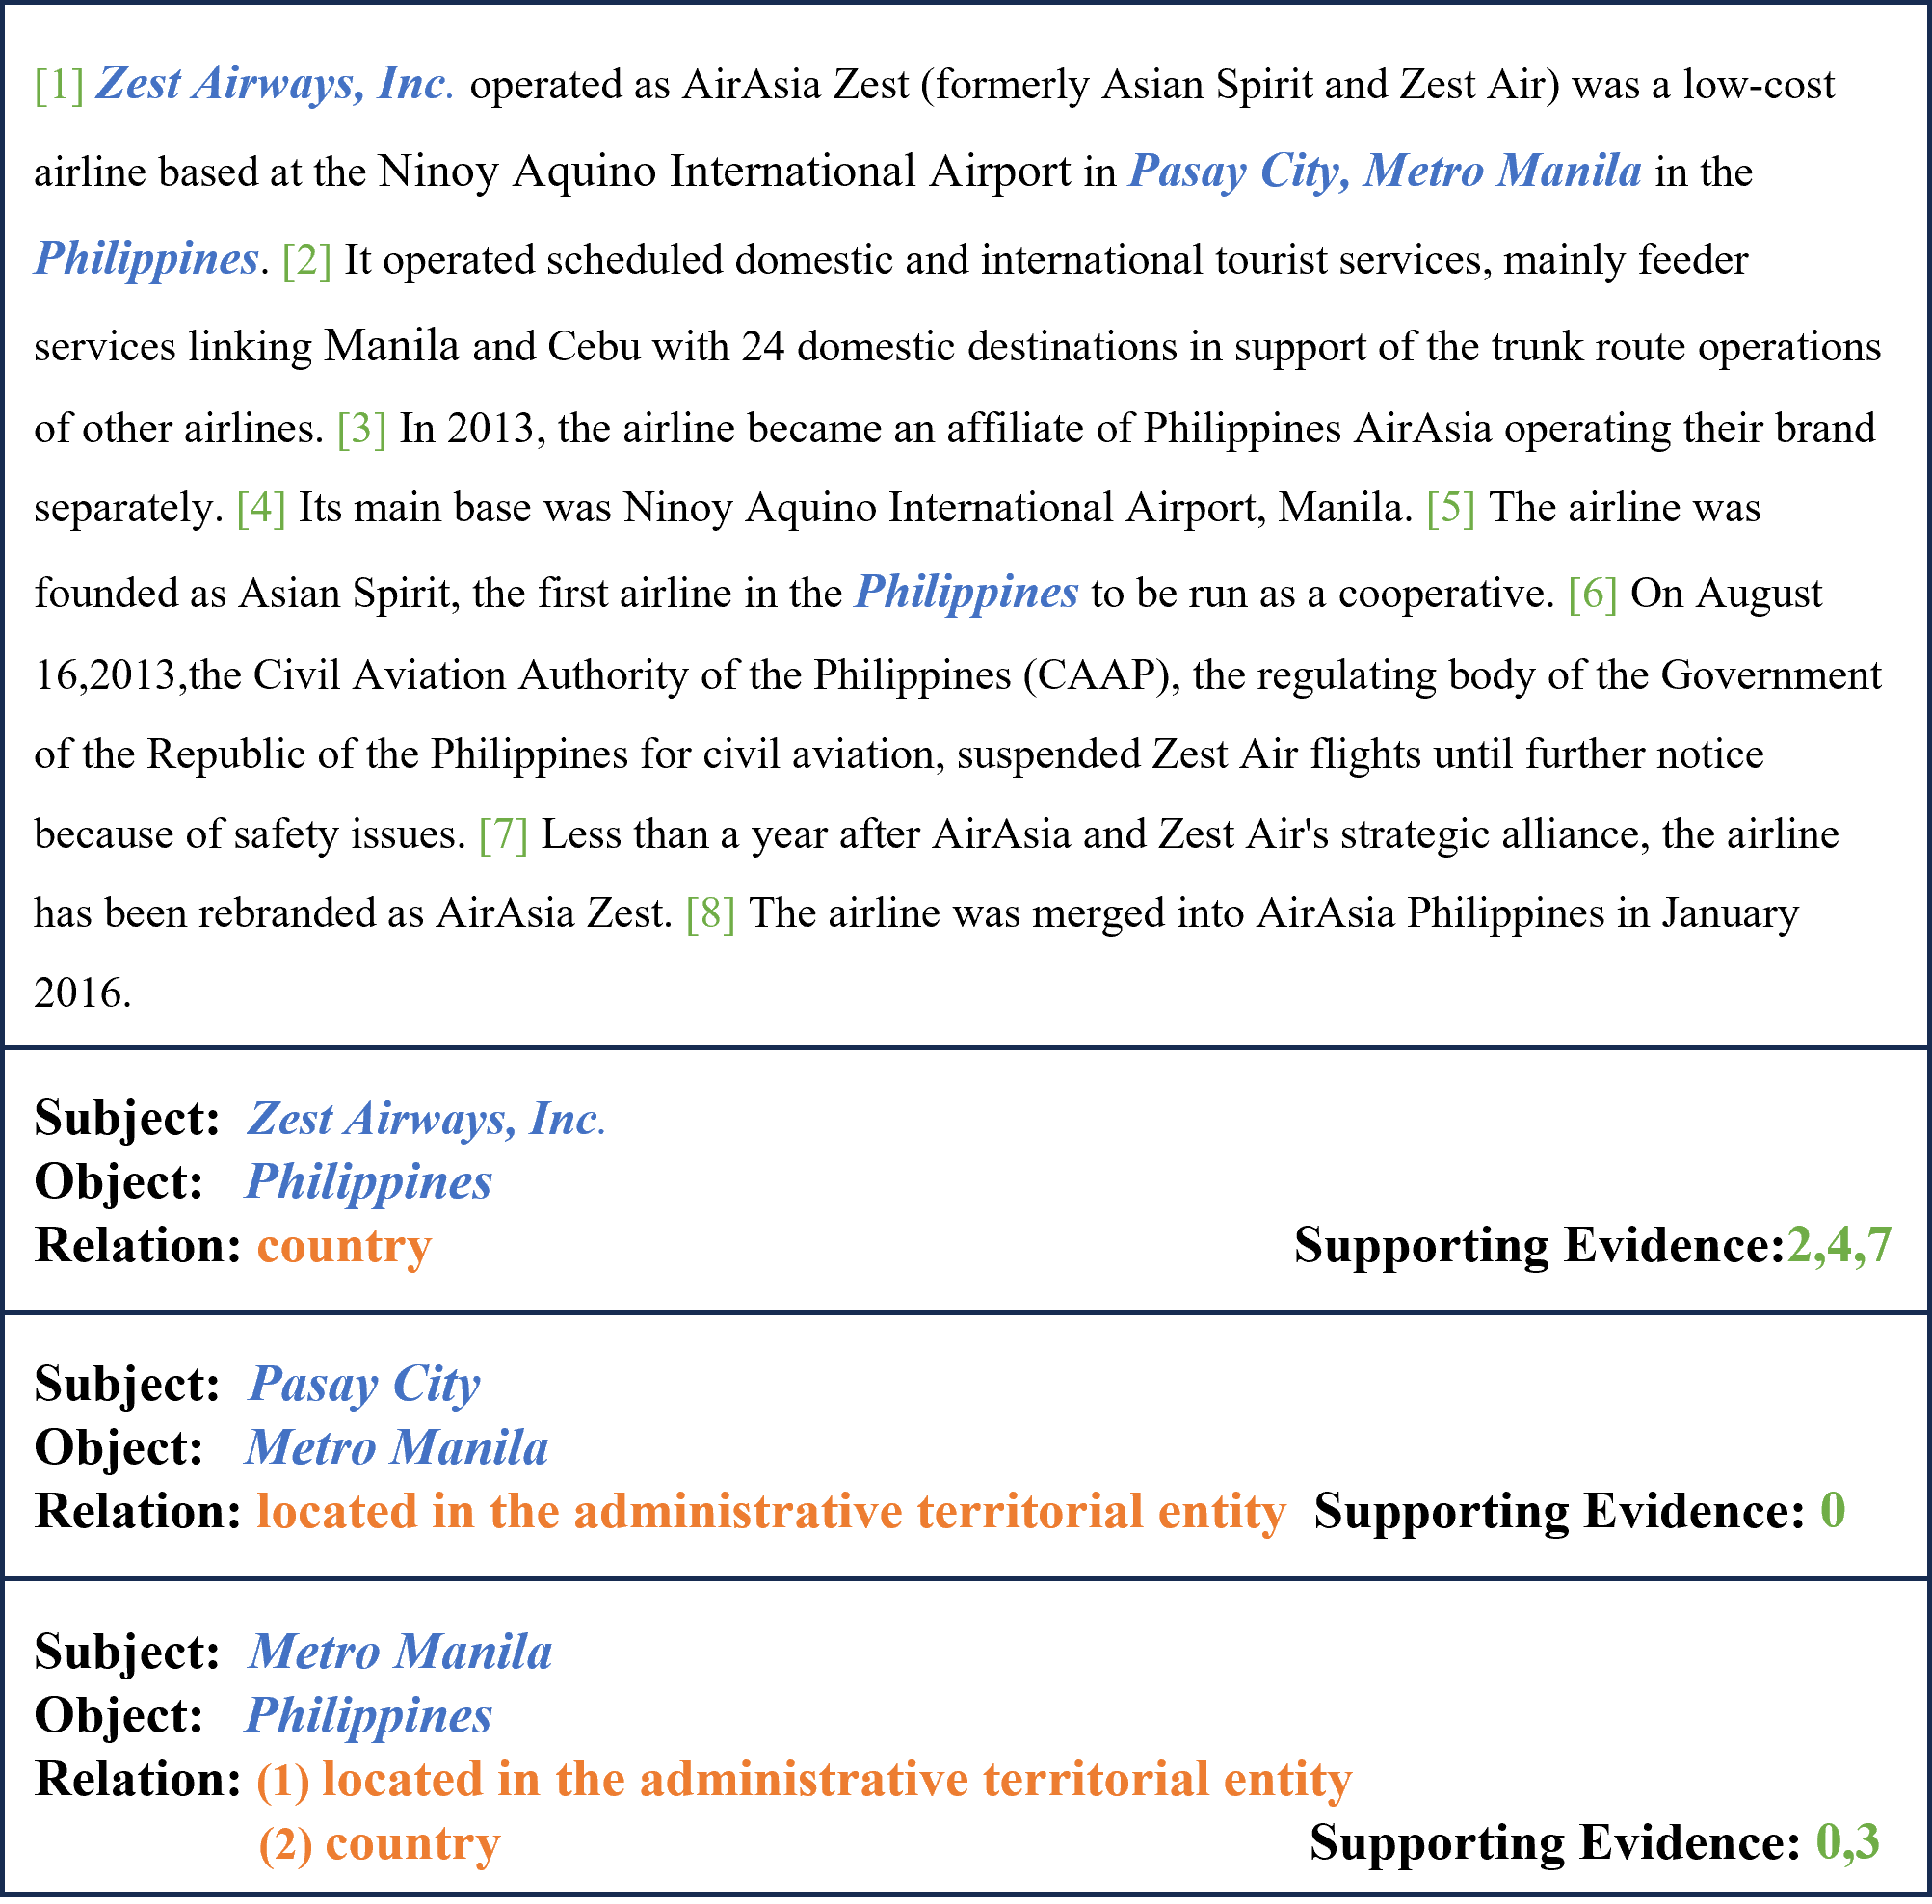
\includegraphics[width=3in]{./dataset.png}
\caption{An example from DocRED. At the beginning of the i-th sentence is marked with a green [i]. Blue bold italics are subject and object entity.}
\label{fig.1}
\end{figure}

Moreover, when solving multiple relations extraction problems with evidence sentences, the DocRE method primarily relies on the semantic information of evidence sentences\cite{huang2021entity,huang-etal-2021-three}, while ignoring the connection of target relations. But the semantic information of evidence sentences may cannot recognize the faint differences between some relations, especially when the target relations are fuzzy and ambiguous\cite{che2022label}.  Therefore, an important problem for most relation extraction methods is that they may just focus on predicting some main relations while ignoring other important relations, which may results in the incomplete relation prediction. Especially in the real applications, such as knowledge graphs and text analysis, incomplete relations will not provide comprehensive information, which will greatly reduce task performance. Hence, we believe that there is an urgent need for a new extraction method, which can both fully utilize the evidence sentence information and consider the connection of target relations to make more accurate prediction, especially when facing multiple relations extraction problem.

In this paper, with respect to the above problems, we propose a multiple DocRE method, named as EG-ReCo. Firstly, the proposed method set heuristic rules to construct a silver evidence set and introduce Reinforcement Learning (RL) to select more effective evidence sentences on the silver evidence. Secondly, we analyze the DocRED dataset and utilize GAT to acquire the features of co-occurrence relations, which can greatly improve multiple relations prediction. In addition, the combination of co-occurrence relation features and evidence sentence information makes our method achieve high effectiveness and accuracy at the same time.

Our contributions are as follows:

-We propose a knowledge distillation framework by utilizing both human-annotated and distantly-supervised datasets. The framework enables the acquisition of a substantial amount of less noisy data, thereby promoting the robustness of relation extraction tasks.

-We introduce RL to further select evidence sentences in the silver evidence set constructed by heuristic rules, which can greatly alleviate the cost of manually annotating evidence sentences.

-We adopt GAT with prior knowledge to capture the features of co-occurrence relations, which can fuse the semantic information of evidence sentences to  greatly improve the prediction performance.

-We conduct a variety of experiments on two DocRE datasets, and the experimental results demonstrate that our method can achieve the state-of-the-art performance. Our code is available at: https://github.com/wanqiy/EG-ReCo
\section{Related works}
\subsection{Document-level relation extraction}\label{subsec2}

Existing methods for DocRE can be broadly divided into two main types. One is to build document-level graphs based on global information and using graph neural networks to predict relations.  Chen et al. \cite{10.1145/3520082} proposed a force-directed graph to comprehensively learn relations, which can capture the global topology of relations. Xu et al.\cite{10.1145/3511808.3557313} reconstructed the original document into a graph structure and designed an efficient path search policy before evidence extraction, reducing the complexity of exploration. The other type employs pre-trained language models (PrLMs) based on the Transformer architecture. Zhao et al.\cite{10.1145/3502223.3502245} utilized PrLMs can implicitly capture long-distance relations, but they overlooked the connection between entity pairs. Therefore, Zhang et al.\cite{ijcai2021p551} constructed entity-level matrices, who utilized semantic segmentation and a U-shaped network to capture local and global information, though its performance is limited by the number of entity pairs in the document. Ma et al.\cite{ma-etal-2023-dreeam} employed distant supervision dataset to increase the number of entity pairs and used a self-training policy to improve the utilization rate of evidence retrieval. Wan et al.\cite{wan-etal-2021-dqn} proposed a deep reinforcement learning-based DQN method for retrieving supporting or refuting evidence to judge the authenticity of relations. Yuan et al.\cite{10.1093/bioinformatics/btae418} built a hierarchical tree diagram (HTG) to integrate key information sources in a document to implement entity-based relational reasoning. Zaratiana et al.\cite{Zaratiana_Tomeh_Holat_Charnois_2024} employ a transformer encoder-decoder architecture with pointing mechanism on a dynamic vocabulary of spans and relation types.

\subsection{Multi-label learning in DocRE}\label{subsec3}

In DocRE tasks, multi-label learning emphasizes the importance of understanding the correlation between different relation labels. Therefore, multi-label learning is often used in multiple relations prediction for DocRE. In complex and realistic texts, the label distribution is often uneven, which may results in the problem of low-frequency relation labels associated with only a few instances\cite{9684942}.Therefore, Wei et al.\cite{wei-etal-2020-novel} proposed a universal framework designed to handle overlapping triplets. However, this method gradually revealed some issues, such as bias exposure, sensitivity to label order, and insufficient generalization capability. Consequently, Zhang et al.\cite{zhang-etal-2021-multi-label-multi} introduced a  sequential relation generation model and took multi-label and multi-hop relation detection as a sequence generation task, which alleviated the model's sensitivity to label order. In order to improve the training efficiency, Sneha et al. \cite{singhania-etal-2023-extracting} combined PrLMs to analyze the potential impact of entity representation methods on generating knowledge of multi-object relations,which transform multiple relations prediction into a ranking selection task. Sakher Khalil et al.\cite{alqaaidi2023multiple} proposed an adaptive multiple relations priority sorting method, which entity labeling step errors may propagate to the relation prediction module. Xie et al.\cite{10.5555/3666122.3667241} proposed a regularization learning framework that includes class-aware thresholds, effectively controlling the allocation of positive and negative pseudo-labels for each class.

\subsection{Comparison and Analysis}\label{subsec4}

In this paper, we propose a novel multiple and knowledge distillation DocRE method. Compared with other document-level relation extraction methods, our method can effectively overcome the problem that global document modeling is easily affected by noise and irrelevant sentence. Specifically, we reduce the effect of noise by using heuristic rules to select potential evidence sentences and then adopting RL to further select evidence sentences. Moreover, we introduced GAT to better capture the relation between global and local information. Compared with other multi-label learning method, we utilize a knowledge distillation framework to combine human-annotated data with distantly-supervised dataset. In addition, our method also adopts multi-level feature fusion strategy to dynamically adjust the weight of relation labels, which greatly improves the prediction accuracy of multi-relation. From these perspectives, these improvements give our method significant advantages in handling multi-relation extraction tasks.



\section{Problem Formulation}
In this section, we present the task formulation for DocRE.  Given a document , comprising \emph{N} sentences and \emph{n} entities, denoted as $\mathrm{D}=\left\{\mathrm{s}_{\mathrm{i}}\right\}_{\mathrm{i}=1}^{\mathrm{N}}$ and entities $\mathrm{E}=\left\{\mathrm{e}_{\mathrm{i}}\right\}_{\mathrm{i}=1}^{\mathrm{n}}$.DocRE often aims to predict all relations between entity pairs $(e_h,e_t)$,where the subscripts denote the subject and object entities. An entity may appear multiple times in the document, and at each time, we call it a mention, defined as $\mathrm{M}=\left\{\mathrm{m}_{\mathrm{i}}\right\}_{\mathrm{i}=1}^{\mathrm{|M|}}$.For each entity pair$(e_h,e_t)$,the task involves predicting relations $R \cup\{\mathrm{NA}\}$, where \emph{R} is the predefined set of relations, and $\mathrm{NA}$ represents no relation. For example, in Fig. 1, entity "Pasay City" and "Metro Manila" consist of an entity pair, and the relations are "located in the administrative territorial entity" and "country" through the evidence sentence (0,3).Formally, we formulate the task as equation (1):
\begin{equation}
R_\tau=P(\tau \mid e_h,e_t)\label{eq1}
\end{equation}
Where $\tau$ is a relational threshold.

\section{Methodology}\label{sec4}
We present a knowledge distillation model architecture, which include a teacher model and a student model. 1)Teacher model: In human-annotated dataset, we use manually annotated data to train a teacher model. 2)student model: we utilize soft labels to train the student model and use human-annotated dataset to fine-tune the trained student model, which describe in detail and shown our method architecture in Fig.\ref{fig.2}: 
\begin{figure}[htbp]
\centering
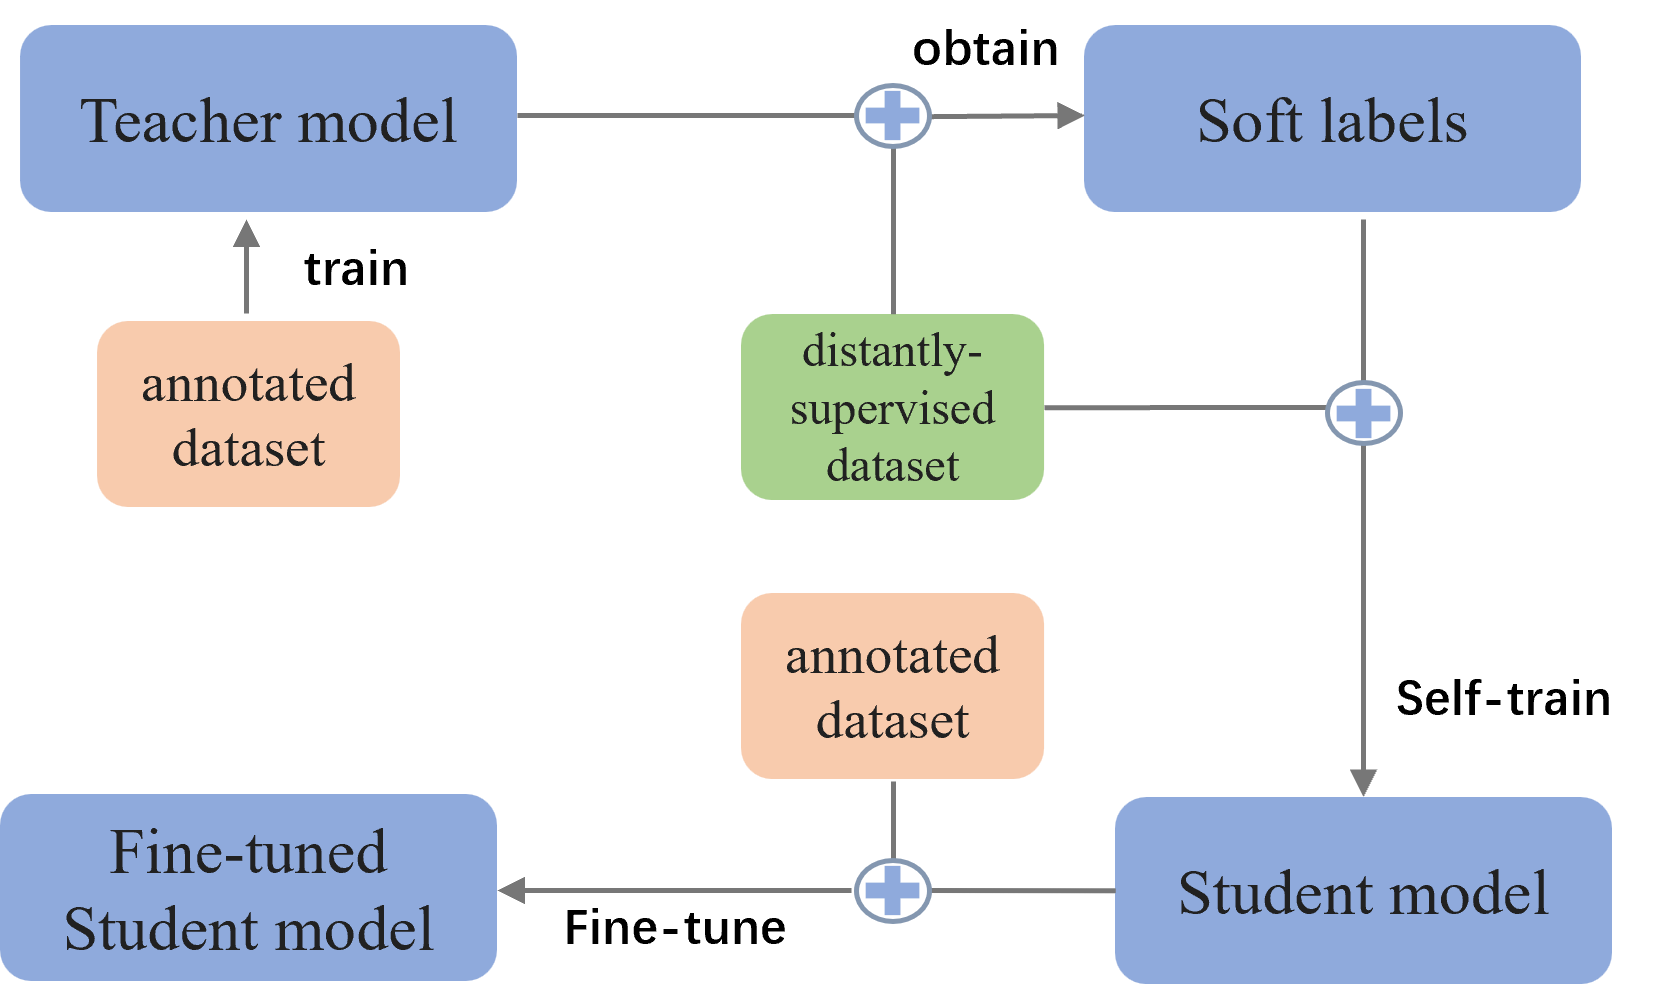
\includegraphics[width=3.5in]{./Flow.png}
\caption{Method Flow.}
\label{fig.2}
\end{figure}

Firstly, the trained teacher model adopts the distant supervision dataset to obtain the probability distribution of the input data prediction, which is called soft label. Soft labels not only contain the predicted relation class but also reflect the confidence of each prediction, which provides a more nuanced supervisory signal than hard labels such as 0 or 1. Secondly, these soft labels are used in the initial training phase of the student model to provide refined supervision signals, so that the student model can learn the probability distribution characteristics of the teacher model. Thirdly, setting heuristic rules to coarse-grained select evidence sentences as the silver evidence set, while introducing RL to fine-grained select more effective evidence sentences in the silver evidence set to gain sentences’ attention. Moreover, these sentences’ attention combines soft labels’ attention to create a new attention for final relations prediction. It is worth noting that, both the teacher model and the student model have the Co-occurrence relations module, where we adopt DREEAM model\cite{ma-etal-2023-dreeam} with above  human-annotated dataset to acquire prior knowledge for calculating the co-occurrence frequency between related relations. In addition, the co-occurrence frequency constructs a comprehensive relation graph to obtain the features of the correlation by GAT. 

Finally, we fine-tune the trained student model using manually annotated dataset. The primary objective of this process is to leverage the knowledge from the teacher model, enhancing the performance of the student model and addressing potential differences between human-annotated dataset and distantly-supervised dataset. In the following sections, we will describe in detail the structure of the teacher model and the student model, the training process in the overall knowledge distillation framework.


\subsection{Teacher model}\label{subsec4}
The document $\mathrm{D}=\left\{\mathrm{s}_{\mathrm{i}}\right\}_{\mathrm{i}=1}^{\mathrm{N}}$ is input into BERT\cite{devlin-etal-2019-bert} to obtain semantic embedding H for each token. Simultaneously, special marker * are added to the left and right sides of the entity, which helps BERT to better understand the location of the entity. Additionally, we calculate multi-head attention \emph{A} to capture intricate dependencies between tokens in the document.

\begin{equation}
H,A= BERT[s_1,s_2 ... s_N]\label{eq2}
\end{equation}
Where is the i-th sentence. For the final encoding \emph{H}, we select the average of the last three layers, in contrast to the method taken by Zhou et al.\cite{zhou2021document}.
\subsubsection{Entities as well as local context encoding}\label{subsubsec1}

Entity embedding $e_s$  is captured through collecting all correspond mentions embedding, which denoted as $\mathrm{M}=\left\{\mathrm{m}_{\mathrm{i}}\right\}_{\mathrm{i}=1}^{\mathrm{|M|}}$. According to the study of Robin Jia et al.\cite{jia-etal-2019-document} , we employ max pooling to obtain the encoded information for entity. 

\begin{equation}
e_{s} = {\log{\sum\limits_{i}^{|M|}{\exp\left( H_{m_{j}} \right)}}}\label{eq3}
\end{equation}
Where $H_{m_{j}}$ represents the embedding at the starting position of mention $m_j$ with a special maker *. In essence, both the head entity $e_h$ and the tail entity $e_t$ have d-dimension encoding vectors, which are calculated to get multi-head attention q for entity pairs. Finally, we integrate these attentions of different entity pairs into whole matrix $q^{(h,t)}$.

\begin{equation}
q^{({h,t})} = \frac{e_{h} \circ e_{t}}{e_{h}^{T}e_{t}}\label{eq4}
\end{equation}
Where ◦ represents the Hadamard product and $q^{(h,t)}$ is a distribution that reveals the importance of each token to the entity pairs $(e_h,e_t)$. Moreover, we utilize local context pooling\cite{zhou2021document} to aggregate separately the importance of the \emph{n} sentences in document \emph{D}:
\begin{equation}
c^{({h,t})} = H^{T}q^{({h,t})}\label{eq5}
\end{equation}
\begin{equation}
Z_{i}^{({h,t})} = {\sum\limits_{j \in {|w_{n}|}}^{w_{n^{'}}}q_{j}^{({h,t})}}\label{eq6}
\end{equation}
Where $H \in \mathbb{R}^{l \times d}$ is the contextual embedding for the entire document. $c^{(h,t)} \in \mathbb{R}^d$ is the weighted average of all token embeddings, and $w_n$ represents the beginning of each sentence in the document, $w_{n'}$ represents its end.


\subsubsection{Co-occurrence relations construction via GAT}\label{subsubsec2}

When two label entities frequently appear together, we consider them to have   co-occurrence relations. We adopt the DREEAM model \cite{ma-etal-2023-dreeam} on the Re-DocRED dataset to obtain  correlation relations distribution. Subsequently, we use the correlation relations distribution to construct a co-occurrence matrix $r^{n*n}(n =97)$.The nodes represent different relation labels (e.g., "Located in," "Part of," and so on). Edges represent the co-occurrence relation between relation labels. Moreover, the weight of the edge is determined by the conditional probability $P\left( L_{i} \middle| L_{j} \right)$,which indicates the probability of label $L_i$ occurring when label $L_j$ is present:
\begin{equation}
P\left( L_{j} \middle| L_{i} \right) = \frac{r_{ij}}{\sum\limits_{j}r_{ij}}\label{eq7}
\end{equation}

However, the above correlation method exists two drawbacks. Firstly, the co-occurrence patterns between relations may exhibit a long-tail distribution, where some rare co-occurrences could be noise. Secondly, when two relations co-occur frequently, the method may be oversensitive to these common co-occurrence relations, instead relatively insensitive to rare co-occurrence relations, which makes the prediction of multiple relations inaccurate. Therefore, we propose to binarize the correlation matrix P and adopt a threshold $\tau$ to filter out noisy edges. This operation can be defined as equation (8):
\begin{equation}
Q_{ij} = \begin{cases}
{0,} & {\text{if~}P_{ij} < \tau} \\
{1,} & {\text{if}{~P}_{ij} \geq \tau}
\end{cases}\label{eq8}
\end{equation}
Where $Q\in R^{n*n}$ is the binarized correlation matrix. However, when using the binarized correlation matrix, which may encounter the issue of excessive smoothing. The issue means that node features might be overly blurred, making it challenging to distinguish nodes from different relations. Therefore, we employ the re-weighted scheme to update node features in the Graph Convolutional Networks(GCN). As shown in the equation (9), the scheme balances self-feature’s node and related to other nodes’ feature by assigning different weights. When the parameter p approaches 1, the weight of the node's self-feature is smaller, on the contrary to emphasize the relation with features of other relevant nodes. Conversely, when p approaches 0, the weight of the node's self-feature is larger, which highlights the node's self-feature while ignoring information from neighboring nodes:
\begin{equation}
\mathbf{Q}_{ij}^{'} = \begin{cases}
{p/\sum_{\begin{array}{l}
{j = 1} \\
{i \neq j}
\end{array}}^{C}\mathbf{Q}_{ij},} & {\text{if~}i \neq j} \\
{1 - p,} & {\text{if~}i = j}
\end{cases}\label{eq9}
\end{equation}

The re-weighting scheme helps preserve the distinctiveness of relations, ensuring that the feature differences between different relations are retained. Thus, we select the GAT network that each node has different weights to transform and integrate the relational features to obtain a new representation G:
\begin{equation}
F_{rel} = f_{1,}f_{2}\ldots f_{n},n = 97
\label{eq10}
\end{equation}
\begin{equation}
H_{rel} = GAT\left( {F_{rel},\mathbf{Q}_{ij}^{'}} \right)
\label{eq11}
\end{equation}
\begin{equation}
G = H_{rel}*W
\label{eq12}
\end{equation}
Where $F_i$ represents the embedding vector of the i-th relation and $\emph{W}$ is a weight matrix used to transform the aggregated features. $H_{rel}$ represents the aggregated feature representation of relations. $G\in R^{r*{d_Q}} $, where r is the number of relations and $d_Q$ is the dimension of each relation feature.

Finally, we will show how GAT contributes to the improvement of multi-relation forecasting by providing concrete examples. For example, an entity pair ("Metro Manila", "Philippines") has only an "entity located in an administrative area" relation in one document, but also contains "entity located in an administrative area" and "country" relations in another document. GAT utilizes the geographic and organizational information between these relations to enhance the model's ability to predict multiple relations. In addition, GAT can dynamically adjust the weight of the edges between relational labels to more accurately capture the global relational network structure in the document.

\subsubsection{Relation Prediction}\label{subsubsec3}
We utilize the above entity embedding and contextual attention embedding to enhance the representations of the head entity $e_h$ and the tail entity $e_t$:
\begin{equation}
\begin{array}{rr}
 & {o_{h} = {\sigma\left( {W_{h}\left\lbrack {e_{h};c^{({h,t})}} \right\rbrack + b_{h}} \right)}} \\
 & {o_{t} = {\sigma\left( {W_{t}\left\lbrack {e_{t};c^{({h,t})}} \right\rbrack + b_{t}} \right)},}
\end{array}
\label{eq13}
\end{equation}
Where $W_h,W_t\in R^{d*2d},b_h,b_o\in R^t$ are trainable parameter and $\sigma$ is the activation function. We obtain the fused feature representation through mapping entity feature vector o and the relation feature, followed by a normalization operation:
\begin{equation}
n_{h} = LayerNorm\left( {G \bullet o_{h}} \right)
\label{eq14}
\end{equation}
\begin{equation}
n_{t} = LayerNorm\left( {G \bullet o_{t}} \right)
\label{eq15}
\end{equation}

Afterward, the new feature vector  $n_i$ is input into a bilinear classifier to calculate the relation transformed score $Y^{(h,t)}$:
\begin{equation}
n_{h}^{'} = n_{h} \oplus o_{h}
\label{eq16}
\end{equation}
\begin{equation}
n_{t}^{'} = n_{t} \oplus o_{t}
\label{eq17}
\end{equation}
\begin{equation}
Y^{({h,t})} = {n_{h}^{'}}^{T}W_{r}n_{t}^{'} + b_{r}
\label{eq18}
\end{equation}
Where $W_r\in R^{(d_Q+r)*(d_Q+r))}$ and $b_r$ are trainable parameters. Finally, we use sigmoid $\sigma$ activation function in $Y^{(h,t)}$ to obtain the probability value $P\left( r \middle| {h,t} \right)$.

\subsubsection{Loss Function}\label{subsubsec4}
During the training process, we comprehensively apply the Adaptive Focal Loss\cite{tan-etal-2022-document}  and  the Adaptive Threshold Loss. Specifically, based on the learned pseudo-threshold class $\emph{TH}$, the loss can be divided into two parts: one for relation prediction loss and the other for evidence sentence loss. In the training of relation prediction, the label space is partitioned into two subsets $N_T$. The $P_T$ encompasses relations associated with entity pairs $(e_h,e_t)$, while the $N_T$  comprises relations not belonging to the positive class. The loss function establishes distinct probability gaps, ensuring that the probability $P\left( r \middle| {h,t} \right)$ for the  $P_T$  is higher than for the  $\emph{TH}$ class and the $N_T$  is lower than the the $\emph{TH}$ class:
\begin{equation}
P\left( {r \mid e_{h},e_{t}} \right) = \frac{\exp\left( Y_{r}^{({h,t})} \right)}{{\exp\left( Y_{r}^{({h,t})} \right)} + {\exp\left( Y_{TH}^{({h,t})} \right)}}
\label{eq19}
\end{equation}

For the  $N_T$,  we utilize  logit to compute the probability $P\left( {r_{TH} \mid e_{h},e_{t}} \right)$ for the $\emph{TH}$ class. In this process, we pay closer attention to low-confidence categories and employ the Focal Loss to balance the logit for positive categories, which contributes to the final equation (20) for the $Loss_r$:
\begin{equation}
P\left( {r_{TH} \mid e_{h},e_{t}} \right) = \frac{\exp\left( Y_{r_{TH}}^{({h,t})} \right)}{\sum_{r_{j} \in \mathcal{N}_{T} \cup \{ TH\}}\,{\exp\left( Y_{r}^{({h,t})} \right)}}
\label{eq20}
\end{equation}
\begin{equation}
\begin{aligned}
\text{Loss}_{r} = & \sum\limits_{r \in P_{T}} \left(1 - P\left(r \mid e_{h},e_{t}\right)\right)^{\tau} \log\left(P\left(r \mid e_{h},e_{t}\right)\right) \\
& + {\log\left( {P\left( {r_{TH} \mid e_{h},e_{t}} \right)} \right)}
\end{aligned}
\label{eq21}
\end{equation}
Where $\tau$ is a hyperparameter. In the evidence sentences loss, we utilize manually annotated golden evidence to supervise the  $Z^{(h,t)}$ for each entity pair $(e_h,e_t)$. For each valid relation label r (including relations in the set associated with the entity pair $(e_h,e_t)$ but excluding unrelated relation NA), a binary vector $v^{(h,r,t)}$ is defined to record whether each sentence w contains evidence information about the relation $(e_h,e_t)$. If the sentence w contains evidence information for some relation, the value of  $v^{(h,r,t)}$ is set to 1; otherwise, set to 0:

\begin{equation}
\mathbf{v}^{(\mathbf{h},\mathbf{t})} = \frac{\sum_{r \in \mathcal{R}_{h,t}}\,\mathbf{v}^{({h,r,t})}}{\sum_{r \in \mathcal{R}_{h,t}}\,1^{\top}\mathbf{v}^{({h,r,t})}}
\label{eq22}
\end{equation}

\begin{figure*}[htbp]
\centering
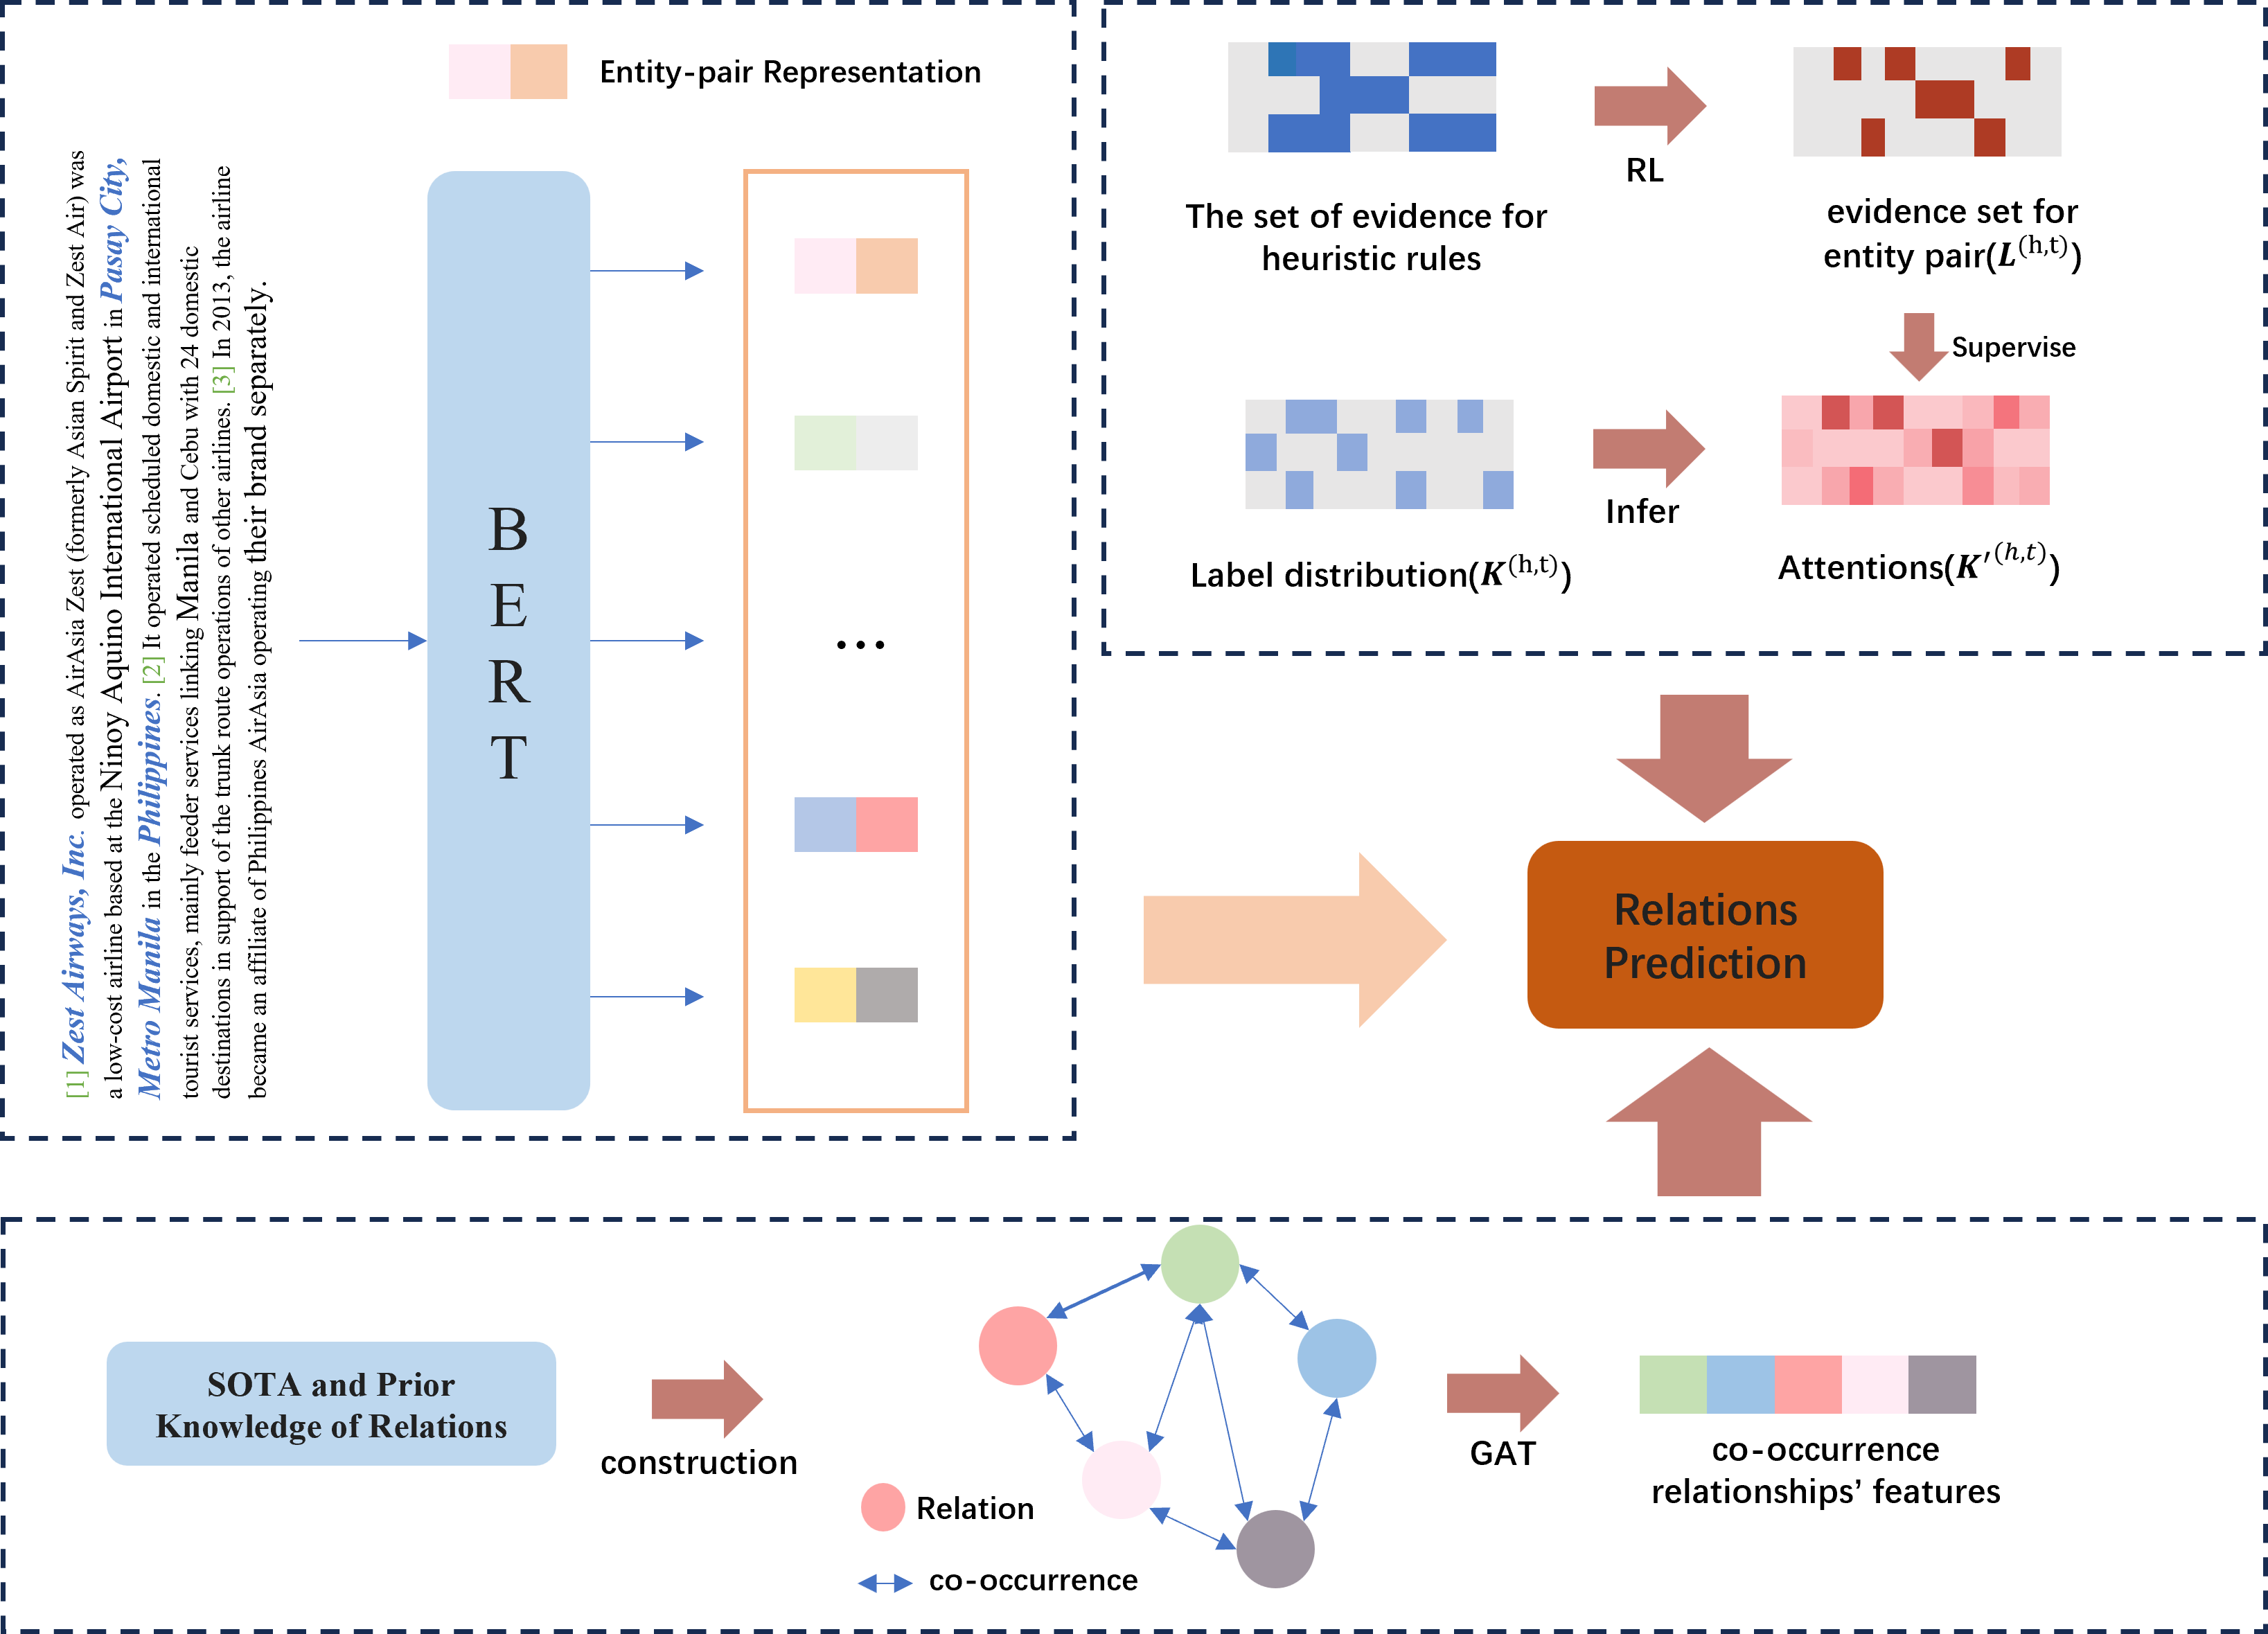
\includegraphics[width=4.5in]{./student_model.png}
\caption{ Internal structure diagram of the student model. The degree of red in $K^{'(h,t)} $ represents the importance of different sentences.}
\label{fig.3}
\end{figure*}
Because the relation prediction not explicitly know the specific relation type, it is necessary to guide the attention module within the encoder to generate token dependencies unrelated to the relation. Therefore, we set a unit vector, which all elements are 1 and $|1|=|w_d|$.We utilize the Kullback-Leibler(KL) divergence loss to train model, which aims to reduce the statistical difference between $Z^{(h,t)}$  and $v^{(h,t)}$ and make them more similar. Finally, we adopt the hyperparameter $\lambda_1$ to balance the impact of relation prediction loss and evidence-guided loss, and the overall $Loss_{sum}$ can be as equation (24):
\begin{equation}
{Loss}_{g} = - D_{KL}\left( Z^{({h,t})} \middle| \middle| v^{(h,t)} \right)
\label{eq22}
\end{equation}
\begin{equation}
{Loss}_{sum} = {Loss}_{r} + \lambda_{1}{Loss}_{g}
\label{eq23}
\end{equation}

\subsection{Student model}\label{subsec2}
Human-annotate datasets are superior in quality, While the dataset’s scale is relatively small and the amount of data is limited. Therefore, we opt to train the student model through employing a larger distantly-supervised dataset\cite{mintz-etal-2009-distant}. However, there exists a issue that the distantly-supervision dataset is without annotated evidence sentences. In order to solve this issue, we employ two methods to obtain labels for evidence sentences. One is using the teacher model to infer the distantly-supervised data, thereby generating a evidence information label distribution $K^{(h,t)}$ for each entity pair $(e_h,e_t)$. Subsequently, the student model is trained for fitting the label distribution to mimic the behavior of the teacher model. The other method is constructing a coarse-grained evidence set through heuristic rules and introducing reinforcement learning to obtain the fine-grained evidence. The specific architecture of the student model is illustrated in Fig\ref{fig.3}.

\subsubsection{Heuristic Evidence Label Construction}\label{subsubsec5}
We devise a set of heuristic rules to automatically construct silver evidence set for evidence extraction, as shown in Fig. \ref{fig.4}.

\begin{figure*}[htbp]
\centering
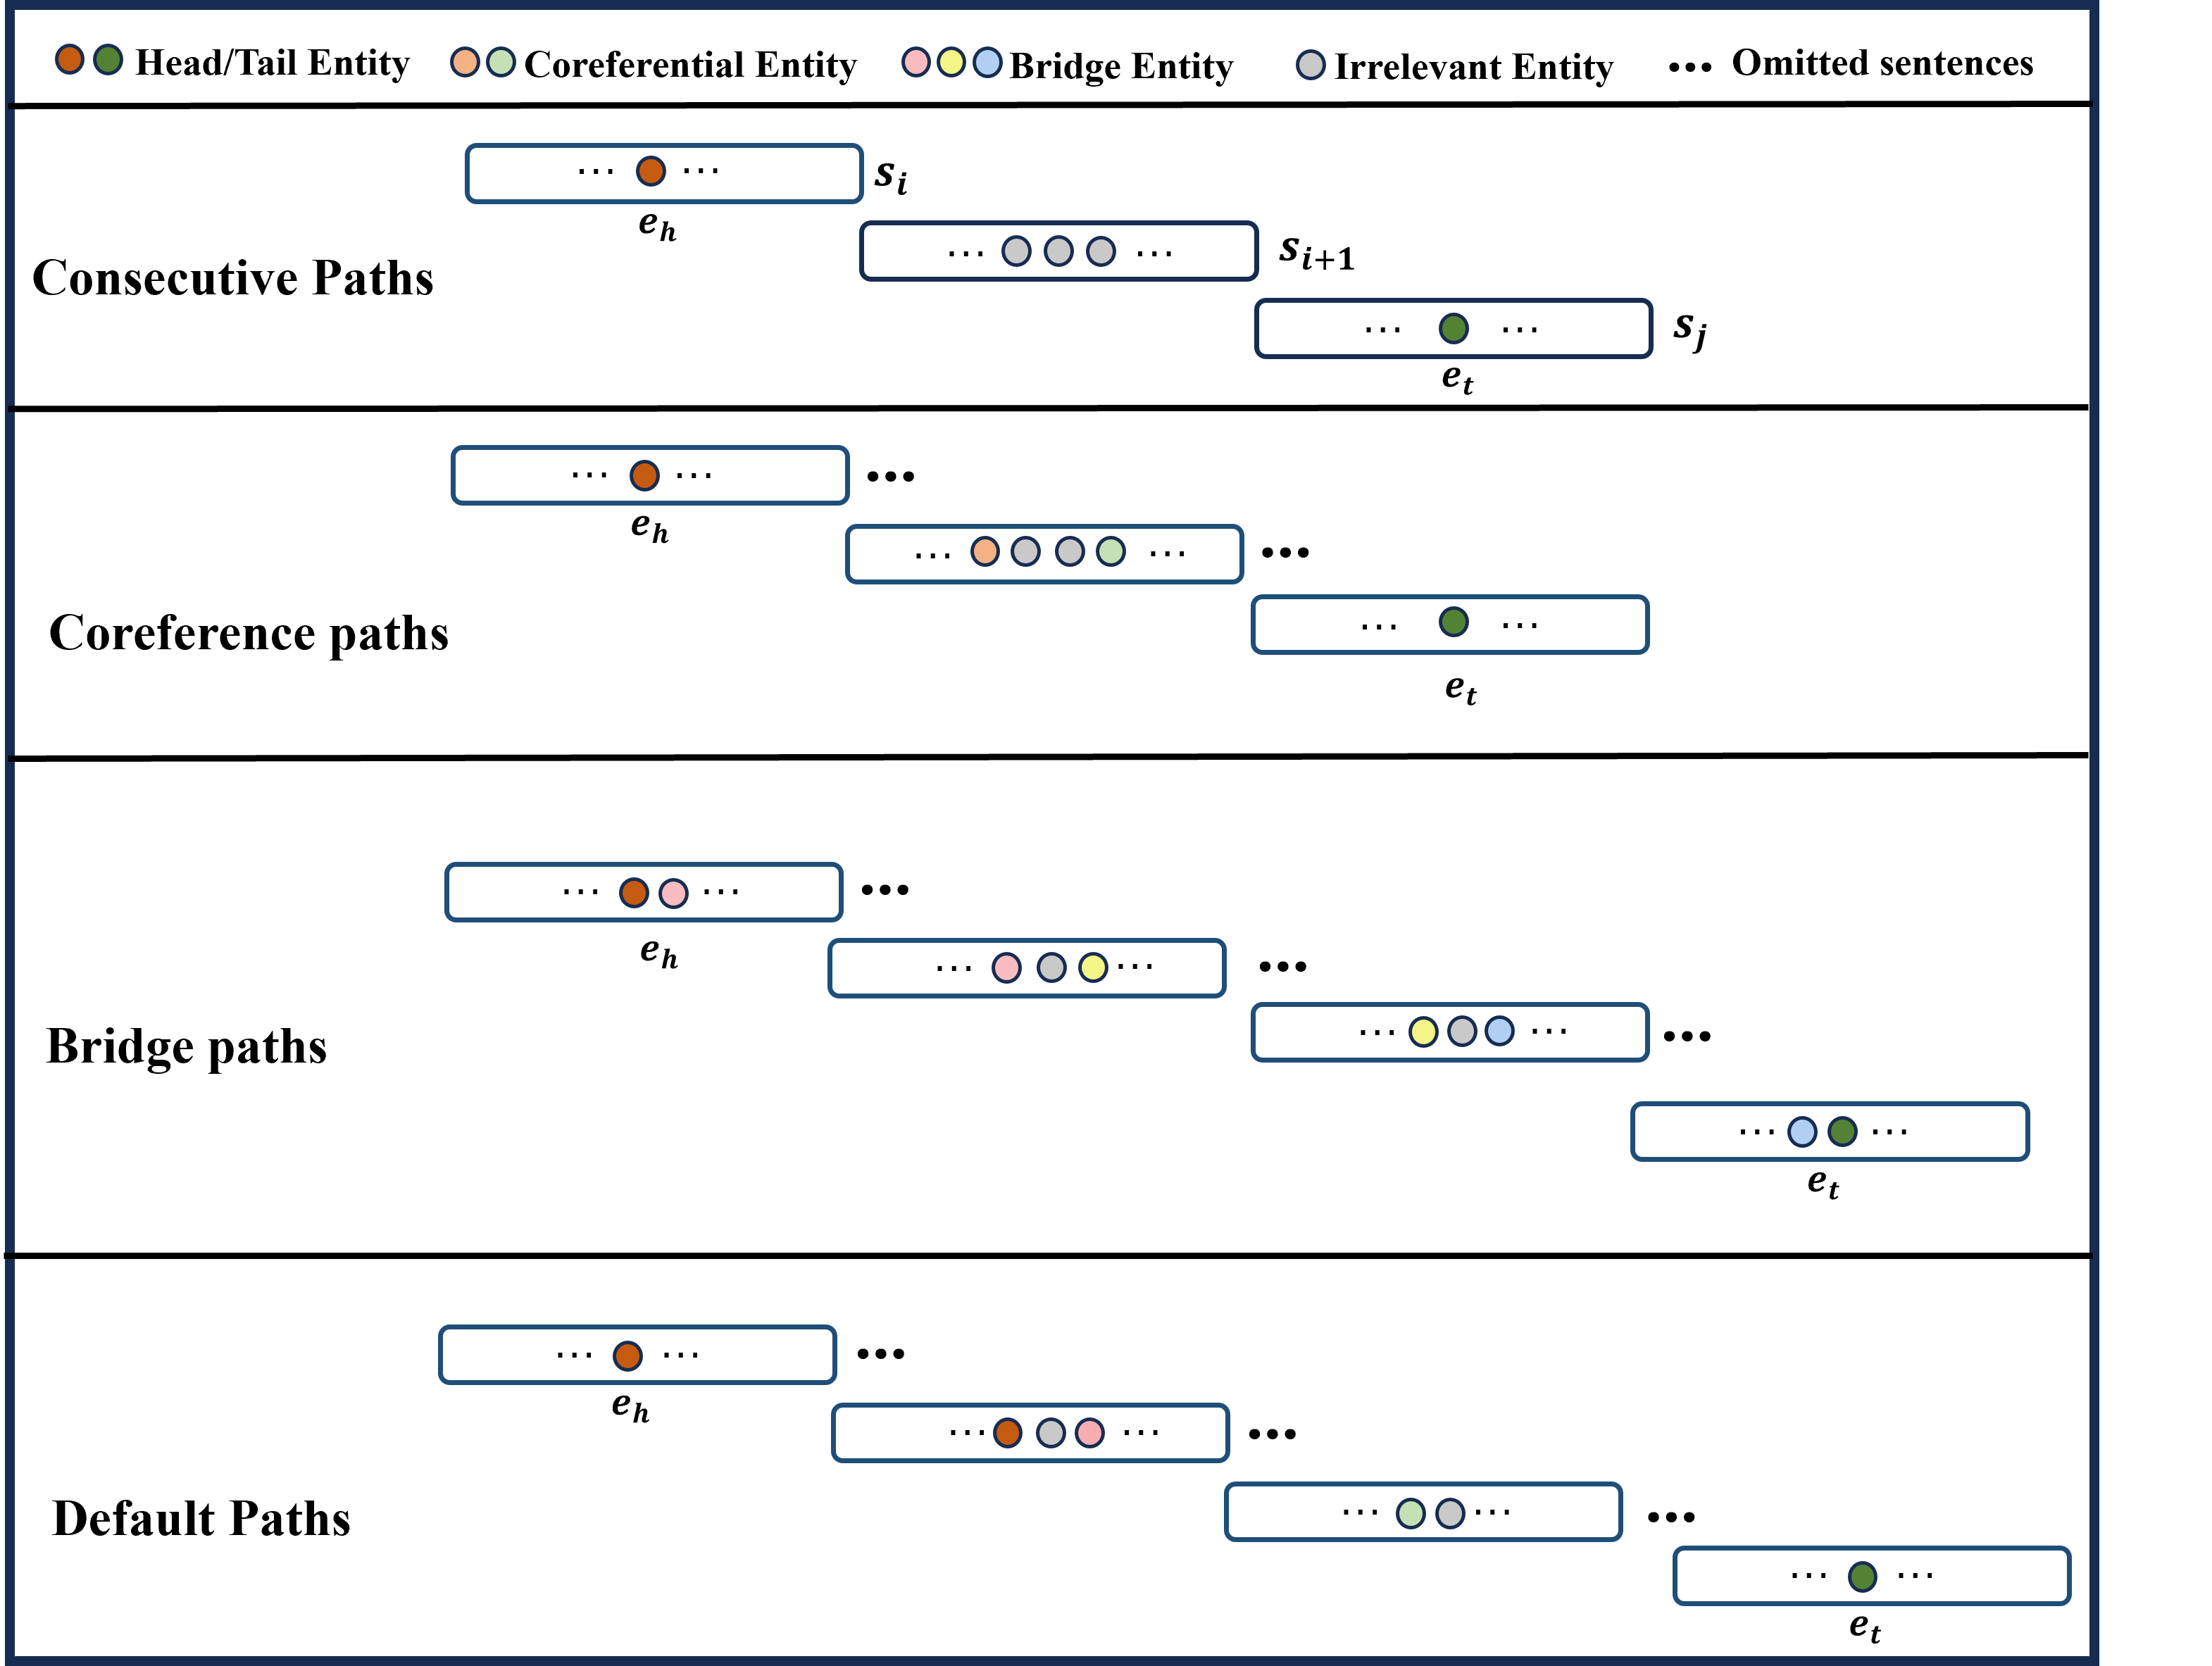
\includegraphics[width=4in]{./path.png}
\caption{ Example diagram of the evidence path. $e_h$ and $e_t$ are the tags of the head and tail entities. $S_i$ is the i-th sentence in the document.}
\label{fig.4}
\end{figure*}
\begin{enumerate}

\item[A.]Consecutive Paths

According to the research presented in\cite{xie-etal-2022-eider}, a few document authors generally use consecutive sentences to describe the relations through continuous sentences. Consequently, there is an observation that most inter-sentence relations can be identified within consecutive sentences. Based on this result, we find a fact that, relations are adequately supported by no more than 3 consecutive sentences. Therefore, we restrict the length of these consecutive paths to a maximum of 3 sentences, i.e., $\mid j-i\le2\mid$. It is essential to note that, this definition naturally applies to cases where the head and tail entities are within the same sentence. Therefore, the same pair of entities can be mentioned multiple times in text, which may be multiple consecutive paths between entities.

\item[B.]Coreference Paths

Given the potential variations in coreferential mentions that same entity of different mentions, we consider all sentences contain coreferential mentions as evidence sentences. Moreover, we can employ a pre-trained Hoi model\cite{xu2021document} to perform co-reference resolution, especially for datasets without explicitly annotated coreference information.
\item[C.]Bridge Paths

In documents, entities often exist an indirect form of association. For example, to express the relation between entity A and entity C, it is necessary to select sentences involving entity A and entity B, as well as sentences involving entity B and entity C. In the case, we refer to entity B as a bridging entity. Typically, the maximum number of bridging entities is limited to two, which result in a maximum of three bridging sentences.
\item[D.]Default Paths

When the head entity and tail entity first appear is not fit the previously mentioned paths, we include the sentence containing the head entity and tail entity first appearance as evidence sentences.
\end{enumerate}

\subsubsection{RL-based Evidence Selection}\label{subsubsec6}
In order to further select the optimal set of evidence sentences on the silver evidence set, we introduce the Reinforcement Learning (RL) framework and adopt the Monte Carlo method for policy evaluation and optimization. Monte Carlo methods evaluate the effectiveness of a strategy by simulating possible evidence selection paths with random sampling and estimating the cumulative rewards of these paths. At the end of each simulation, the strategy is updated based on the cumulative reward, so that the model can more accurately select the evidence sentences that support relation prediction. This method not only improves the robustness and prediction accuracy of the model, but also reduces the interference of irrelevant information. In addition, through the continuous optimization strategy, the model can adaptively select the most representative evidence sentences in different documents, which significantly improves the overall performance of multi-relation extraction. Finally, we will explain how RL is implemented in detail from the five aspects of State, Action, Reward, Policy, Optimization and framework of evidence extraction as shown in Fig.\ref{fig.5}.

\begin{figure*}[htbp]
\centering
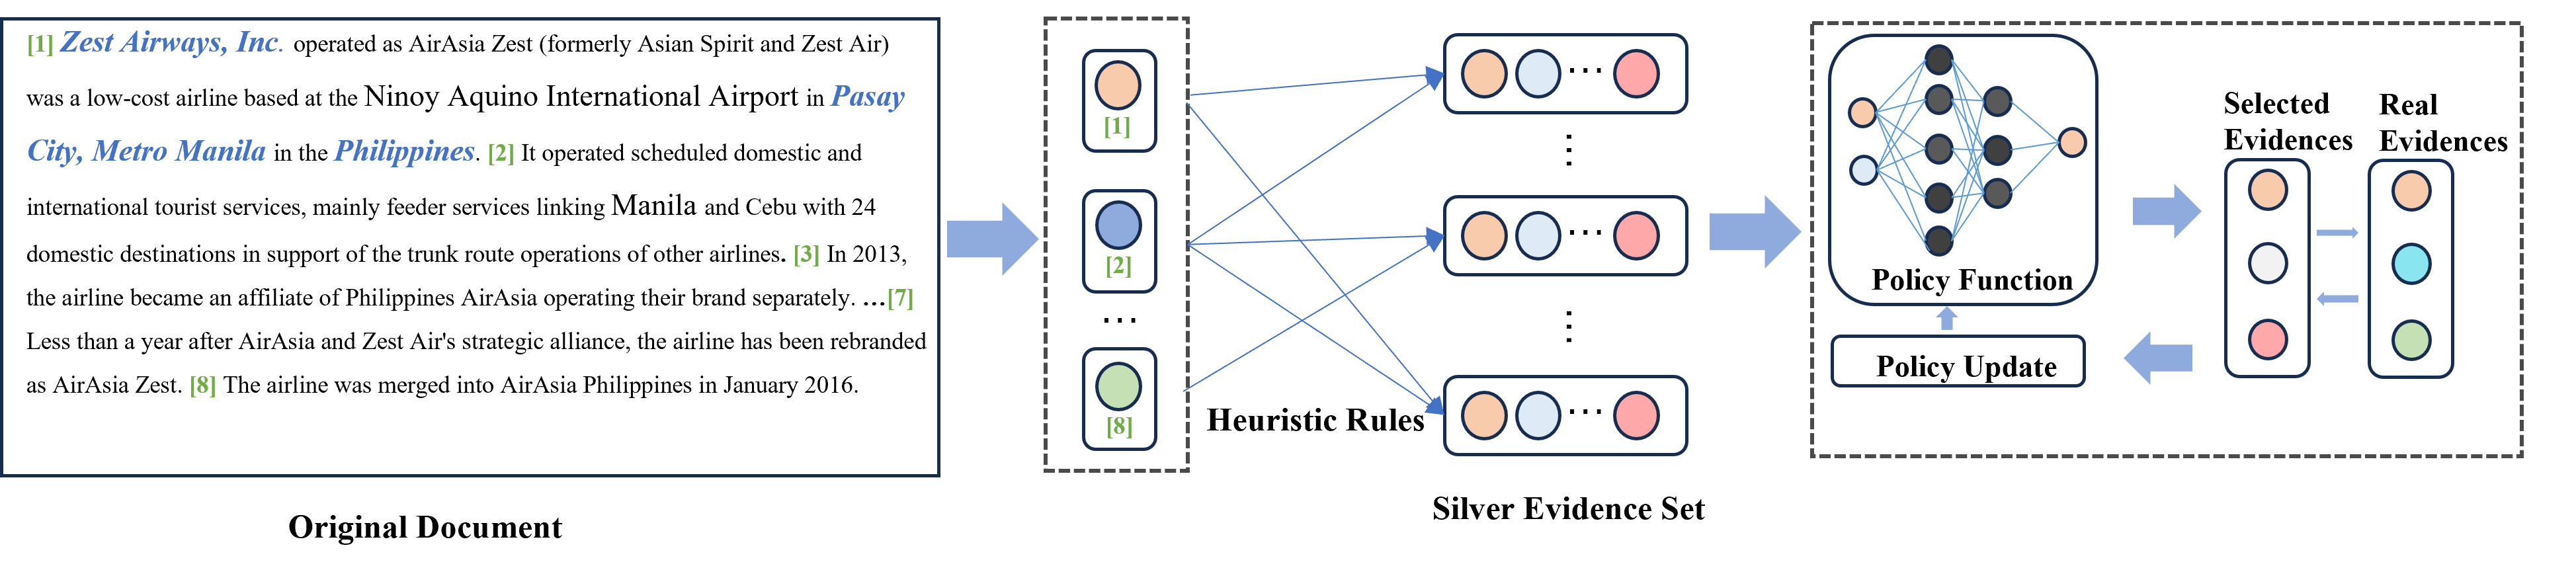
\includegraphics[width=5.5in]{./RL.png}
\caption{ Framework of evidence extraction.}
\label{fig.5}
\end{figure*}

\begin{enumerate}
\item[A.]State 

 We fuse the head entity embedding $e_{h}$ and tail entity embedding $e_{t}$ for each entity pair,while introducing contextual dependencies $c^{(h,t)}$ and sentence information $st_i$:
\begin{equation}
{st}_{i} = mean\left( {\sum\limits_{i \in {|n|}}s_{i}} \right)
\label{eq24}
\end{equation}
\begin{equation}
S = \left\lbrack {e_{h} \oplus e_{t} \oplus c^{({h,t})} \oplus {st}_{i}} \right\rbrack
\label{eq25}
\end{equation}

Because the crucial requirement of Markovian property in reinforcement learning, the current selection of evidence sentences impacts future selections. To meet with the above requirement, if a sentence is an evidence sentence by using state $S$, the next sentence from the pseudo-document is concatenated in the current state $S$. If the predicted sentence is not an evidence sentence, rollback to the previous state. Therefore, the state can be defined with a quadruple: head entity embedding $e_h$, tail entity embedding $e_h$, the entity pair's contextual dependencies $c^{(h,t)}$ and information about the current sentence information in the evidence set $st_i$.

\item[B.]Action

Each pair of entities corresponds to an evidence set, where sentences are filtered by heuristic rules. Monte Carlo method is used to select the sentence with the highest probability as the outcome in the evidence set. The sample implies that the number of evidence sentences for each entity pair is not fixed. Additionally, we retain the probability for reward:

\begin{equation}
a = \left\{ \begin{matrix}
{1,if{~\pi}_{q}\left( {s,a = 1} \right) \geq {~\pi}_{q}\left( {s,a = 0} \right)} \\
{0,otherwise}
\end{matrix} \right.
\label{eq26}
\end{equation}
Where $\pi_{q(s,a=1)}$ represents the probability of an evidence sentence under the predefined policy, while $\pi_{q(s,a=0)}$ represents the probability of a non-evidence sentence.

\item[C.]Reward

For Monte Carlo method, the agent does not immediately receive rewards after taking actions. Instead, the reward is generated only at the end of each episode for each entity pair. So, the reward can be defined as equation (28):
\begin{align}
r(S_{i} \mid D_{\tau}) = 
\begin{cases}
\begin{aligned}
&0 \quad \text{if } i < |D_{\tau}| + 1 \\
&\frac{1}{|\Phi|}\sum_{i=1}^{n} \biggl[ y_{i} \cdot \log\left( 1 - P(y_{i} \mid X) \right) \\
&\quad + (1 - y_{i}) \cdot \log\left( P(y_{i} \mid X) \right) \biggr] \quad \\ &\text{if } i = |D_{\tau}| + 1
\end{aligned}
\end{cases}
\end{align}


\item[D.]Policy

Policy is the decision-making mechanism in RL to guide the agent's interactions with the environment for maximize cumulative rewards or achieve specific goals. The policy can be formally defined as a mapping function that maps states to a probability distribution of actions. Here, the policy can be defined as equation (29):
\begin{equation}
\pi_{q}\left( {s,a} \right) = a \bullet \sigma\left( {\omega*s + \vartheta} \right) + \left( {1 - a} \right) \bullet \left( {1 - \sigma\left( {\omega*s + \vartheta} \right)} \right)
\label{eq29}
\end{equation}
Where $\sigma$ is an activation function, and $\omega,\vartheta$  are  two trainable parameters.

\item[E.]Optimization

We employ the REINFORCE algorithm to train the agent for an optimized policy. The policy aims to adjust $Q$ values from a neural network by maximizing the expected cumulative rewards. Moreover, according to the policy gradient theorem, the policy gradient $
\nabla J(\theta)$ can be defined as equation (30):
\begin{equation}
\nabla J(\theta) = \nabla{\log{\pi_{q}\left( {s,a} \right)}} \bullet v
\label{eq30}
\end{equation}
Where $v$ represents the cumulative reward for the state-action pair $(s,a)$ , which is considered an unbiased estimate of $Q_{\pi(s,a)}$. Therefore, for each state $s$, the update of parameters $\theta$ can be defined as equation (32). The updating process helps the agent continuously improve the policy to maximize the expected cumulative reward:
\begin{equation}
v_{i} = \gamma^{{|D_{\tau}|} + 1 - i} \bullet r\left( {s_{{|D_{\tau}|} + 1}\left| D_{\tau} \right|} \right)
\label{eq31}
\end{equation}
\begin{equation}
\left. \theta\leftarrow\theta + \alpha\nabla J(\theta)v_{i} \right.
\label{eq32}
\end{equation}
Where learning rate $\alpha$ is used to control the update rate of parameters $\theta$. Where $\gamma$ is the reward discount factor, which determine the relative importance of future rewards. Consequently, we obtain the labeled distribution $L^{(h,t)}$ for the entity pair's silver evidence set through RL. Finally, $L^{(h,t)}$ is combined with $K^{(h,t)}$ to form a new labeled distribution $K^{'(h,t)}$for the entity pair's evidence set, which can be represented as equation (33):
\begin{equation}
{K^{'}}^{(h,t)} = \left( {1 - \lambda_{2}} \right)K^{(h,t)} + {\lambda_{2}L}^{({h,t})}
\label{eq33}
\end{equation}

Where $\lambda_2$ is variable parameter.Finally, in order to show the RL method in the evidence selection process more intuitively, we provide pseudo-code as shown Algorithm 1, which describes the specific operation and decision basis of each step in detail.

\begin{algorithm}[H]
\small
\caption{Monte Carlo-based Training Procedure for Evidence Selection}
\KwData{An empty experience memory $M$ with a capacity of $N$}
\KwResult{Refined evidence set $T$ selected from the silver evidence set}

Initialize the policy $\pi$ randomly\;
Set the maximum number of episodes $E$ and the maximum number of evidence sentences $K$\;

\For{episode = 1 to $E$}{
    Get silver evidence set $C$ for target entity pairs using heuristic rules\;
    Initialize the starting state $S$ with head entity embedding $e_h$, tail entity embedding $e_t$, contextual dependencies $c^{(h,t)}$, and sentence information $st_i$\;
    Initialize the evidence set $T$ as empty\;
    
    \For{$t = 0$ to $K$}{
        Select an action $a_t$ (select a sentence as evidence) using the current policy $\pi_q(s,a)$\;
        Update the evidence set $T_{t+1} = T_t \cup \{a_t\}$\;
        Update the state $s_{t+1}$ with the new action $a_{t+1}$\;
        
        \If{random() $< \epsilon$}{
            Select a random action $a_{t+1}$ where $a_{t+1} \in C$\;
        }
    }
    
    Calculate the cumulative rewards $R$ for the selected evidence set $T$\;
    Store the episode $(s, a, R)$ in the experience memory $M$\;
    Update the policy $\pi$ using the episodes stored in $M$ to maximize expected cumulative reward\;
}
\Return{the refined evidence set $T$ selected from the silver evidence set}\;
\end{algorithm}
\end{enumerate}


\subsubsection{Fusing Evidence Set}\label{subsubsec7}
The selected sentences contain the most of information related to the relations in evidence set, While the evidence set may not encompass all information. Therefore, we consider fusing  the original document D and RL-based evidence set $D'$ to obtain complete information. If relations exist  in both the original document and the evidence set, and the prediction scores are positive in both cases,  we add relations to the final merged result. For relations appearing only in the original document or evidence set, we handle the score $S_{(title,h,t,r)}$ to further filter relations prediction results. Based on the score ranking, we select relations with scores above the threshold as predictive outcomes. The fusion policy $P_{(title,h,t,r)}$ can be defined as equation (34) and the loss function $\mathcal{L}_{\text{F~}}$  can be defined as equation (35):
\begin{equation}
P_{({title,h,t,r})} = \sigma\left( {S_{D{({title,h,t,r})}} + S_{D^{'}{({title,h,t,r})}} - \tau} \right)
\label{eq34}
\end{equation}
\begin{equation}
\begin{matrix}
{\mathcal{L}_{\text{F~}} = - \sum_{d \in \mathcal{D}}\,\sum_{h \neq t}\,\sum_{r \in \mathcal{R}}\,y_{r} \cdot P_{(title,h,t,r)\ } +} \\
{\left( {1 - y_{r}} \right) \cdot {\log\left( {1 - P_{{({title,h,t,r})}\ }} \right)}}
\end{matrix}
\label{eq35}
\end{equation}
Where $\sigma$ denotes the aggregation in the fusion layer of two sets of prediction results and $\tau$ represents a learnable parameter. Where  $y_r$ is a binary variable, which takes the value 1 if the relations $r$ between $(e_h,e_t)$ is correctly predicted to exist, and 0 otherwise.


\section{Experiments}\label{sec5}
\subsection{Experiment Preparation}\label{subsec3}
\subsubsection{Datasets}\label{subsubsec7}
We utilize two DocRE benchmark datasets, which contain the DocRED dataset and the revised Re-DocRED dataset\cite{tan-etal-2022-revisiting}. The specific details are outlined in Table \ref{tab1}.


{\bf{DocRED\footnote{Data set download URL:https://github.com/thunlp/DocRED.}:}} The DocRED is a large-scale document-level relation extraction dataset consisting of 5,053 Wikipedia documents covering 132,375 entities and 56,354 relation facts across 96 different relation types. The dataset includes 3,053 instances for training and 1,000 instances for validation. These documents cover a wide range of topics and domains and provide a rich sample of contexts and relations, which helps to study diversity and complexity in relation extraction. A notable feature of DocRED is the availability of a large amount of remotely supervised data, which aims to support weakly supervised relation extraction research. During data preprocessing, we first deduplicated and cleaned the raw text to remove irrelevant HTML tags and formatting errors. Then, the entity is standardized to ensure consistency of entity representation, and the inconsistent entity references are corrected by matching algorithm.
 
{\bf{RE-DocRED\footnote{Data set download URL: https://github.com/tonytan48/Re-DocRED.}:}} To address the issue of false negative problem caused by incomplete labeling in the DocRED dataset, Tan et al. [28] systematically revised the dataset and proposed an improved dataset Re-DocRED. In addition, the revised dataset addresses incompleteness by supplementing numerous relation triplets, which resolves logical inconsistencies and corrects core errors within DocRED. The dataset of Re-DocRED is divided into 1,000 evaluation documents, of which 500 are used for validation and 500 for testing, ensuring the reliability and coverage of the evaluation. In the data preparation phase, we conducted further data cleaning of Re-DocRED to eliminate redundant information, and the accuracy of the newly added and revised relation triples was verified through a combination of automated scripts and manual review.
 

\subsubsection{Evaluation Metrics}\label{subsubsec8}
We employ a variety of evaluation metrics to comprehensively evaluate the performance of the model, including $F_1$, $lgn F_1$, precision, recall and $Evi$ $F_1$ score. $F_1$ score is a common metric in relation extraction tasks, which measures the comprehensive performance of the model on all relation types by the harmonic mean of precision and recall. We also utilize the $lgn F_1$ score to evaluate the prediction of those relations that appear in the validation or test set but are not present in the training set, as a measure of the model's ability to generalize when dealing with unseen relations. For the evidence extraction part, we calculated $Evi$ $F_1$score and $Pos$ $Evi$ $F_1$ score to measure the model's effect on extracting evidence sentences for all entity pairs and evidence sentences for positive sample entity pairs. The calculation method of  $Evi$ $F_1$ score depends on the match between the predicted evidence sentences and the actual evidence sentences, including the number of correctly predicted evidence sentences, the number of incorrectly predicted evidence sentences and the number of missed actual evidence sentences, so as to obtain the precision and recall rate, and further calculate the $F_1$  score, which can be represented as equation (36):
\begin{equation}
{E v i F_1=2 \times \frac{E v i_{\mathrm{P}} \times E v i_{\mathrm{R}}}{E v i_{\mathrm{P}}+E v i_{\mathrm{R}}}}
\label{eq33}
\end{equation}

\subsubsection{Implementation Details}\label{subsubsec8}
We employ BERT as the pretraining model and manually adjust all hyperparameters. In training teacher model phase and training student model phase, the learning rate is set to 5e-5, training epochs as 30. The warm-up policy is applied to the initial 6\% steps, while the maximum gradient norm is clipped to 1.0. In the soft labels phase, the learning rate is set to 3e-5 and 2 epochs of training. The learning rate for the fine-tuning phase is set to 1e-6 and the model is trained for 10 epochs. For each phase, the $\lambda$ value is grid searched from [0.1, 0.15, 0.2, 0.25], where $\lambda_1$ is initialized to 0.1 and $\lambda_2$ is initialized to 0.2. The threshold for evidence sentence filtering is selected from the range [0.1, 0.15, 0.2, 0.25], and the final threshold is set to 0.2. 

We train and evaluate EG-ReCo on four Tesla P100 16GB GPU and select the best-performing model on the validation set for predicting the test set, while submitting the predictions to CodaLab for evaluation \footnote{https://codalab.lisn.upsaclay.fr/competitions/365. Submissions under username “wanqizi”are from this work.}.

\subsection{Experimental analysis}\label{subsec4}
\subsubsection{Baselines}\label{subsubsec9}
We compare our method with other methods on the CodaLab leaderboard, including methods based on graphs and Transformers. Notably, ATLOP, KD, FCDS and AA lack evidence extraction capabilities. Table \ref{tab2} and Table \ref{tab3} list the performance of the proposed and existing state-of-the-art methods on the DocRED and Re-DocRED datasets. We chose the average of the five experimental results as the result.

\begin{table}[h]
\centering
\caption{Statistics of Re-DocRED and DocRED.}\label{tab1}
\resizebox{10cm}{!}{%
\begin{tabular}{lcccccc}
\hline
Dataset & \multicolumn{3}{c}{Re-DocRED} & \multicolumn{3}{c}{DocRED} \\ 
& Train & Dev & Test & Train & Dev & Test \\
\hline
Documents  &  3053 & 500 & 500 & 3053 & 1000 & - \\
Avg. Entities  & 19.4 & 19.4  & 19.6 & 19.5 & 19.6 & - \\
Avg. Triples  & 28.1 & 34.6  & 34.9 & 12.5 & 12.3 & - \\
Avg. Sentences  & 7.9 & 8.2  & 7.9 & 7.9 & 8.1 & - \\
\hline
\end{tabular}%
}
\end{table}


\begin{table*}[h]
\centering
\caption{Results on the development and test sets of DocRED. DocRED's test set is on CodaLab}\label{tab2}
\begin{tabular*}{\textwidth}{@{\extracolsep\fill}lcccccc}
\hline
Model & \multicolumn{3}{c}{Dev} & \multicolumn{3}{c}{Test} \\
& $lgn$ $F_1$ & $F_1$ & $Evi$ $F_1$ & $lgn$ $F_1$ & $F_1$ & $Evi$ $F_1$ \\
\hline
E2GRE\cite{huang2021entity} & 55.22 & 58.70 & 44.07 & 48.78 & 51.06 & 43.83 \\
ATLOP\cite{zhou2021document} & 59.22 & 61.09 & - & 59.31 & 61.30 & - \\
EIDER\cite{xie-etal-2022-eider} & 60.51 & 62.48 & 50.71 & 60.42 & 62.47 & 51.27 \\
KD-DocRE\cite{tan-etal-2022-document} & 63.38 & 64.81 & - & 62.56 & 64.76 & - \\
FCDS\cite{zhu2024fcds} & 62.61 & 64.42 & - & 62.08 & 64.21 & - \\
AA\cite{lu-etal-2023-anaphor} & 61.31 & 63.38 & - & 60.84 & 63.10 & - \\
$DREEAM_{teacher}$\cite{ma-etal-2023-dreeam} & 59.60 & 61.42 & 52.08 & 59.12 & 61.13 & 51.71 \\
$DREEAM_{student}$\cite{ma-etal-2023-dreeam} & 63.92 & 65.83 & 55.68 & 63.73 & 65.87 & 55.43 \\
\hline
$\mathbf{EG-ReCo_{teacher}}$ & 60.44 & 62.07 & 52.88 & 60.82 & 62.11 & 52.38 \\
$\mathbf{EG-ReCo_{student}}$ & $\mathbf{64.51}$ & $\mathbf{66.34}$ & $\mathbf{56.23}$ & $\mathbf{64.39}$ & $\mathbf{66.56}$ & $\mathbf{56.69}$ \\
\hline
\end{tabular*}
\end{table*}


\begin{table*}[h]
\centering
\caption{Results on the development and test sets of Re-DocRED. There is no Evi F1 index in other corresponding papers, it is not evaluated in the Re-DocRED dataset.}\label{tab3}
\begin{tabular*}{\textwidth}{@{\extracolsep\fill}lcccc}
\hline
Model & \multicolumn{2}{c}{Dev} & \multicolumn{2}{c}{Test} \\
& $lgn$ $F_1$ & $F_1$ & $lgn$ $F_1$ & $F_1$ \\
\hline
ATLOP\cite{zhou2021document} & 73.23 & 73.97 & 73.50 & 74.34 \\
KD-DocRE\cite{tan-etal-2022-document} & 73.57 & 74.14 & 73.66 & 74.44 \\
DREEAM\cite{ma-etal-2023-dreeam} & 74.17 & 75.11 & 75.11 & 75.29 \\
$\mathbf{EG-ReCo}$ & $\mathbf{76.63}$ & $\mathbf{77.46}$ & $\mathbf{76.57}$ & $\mathbf{77.32}$ \\
\hline
\end{tabular*}
\end{table*}



\subsubsection{ Analysis on RL selected Evidence Paths}\label{subsubsec10}
In the realm of relation extraction tasks, the coverage rate of evidence sentences emerges as a pivotal metric for assessing model performance. The rate represents the proportion of model-generated evidence sentences compared to manually annotated crucial information sentences in a dataset. In addition, the rate directly reflects the model's capability to capture key information in relation extraction tasks. A high evidence sentence coverage rate signifies that the model can comprehensively capture information in the text relevant to relations between entity pairs.

However, a high coverage rate does not inherently ensure the quality of the evidence set, as generated evidence sentences may contain redundancies in practical scenarios. Therefore, we introduce RL to enhance the precision of the evidence set and reduce redundant information. Through RL, our method learns how to select the most informative evidence sentences in specific contexts, and thereby further enhance the sentence precision. RL optimizes our method's decision-making process, which enables more intelligent evidence selection and effectively reduces redundant information, thereby improving the overall quality of the evidence set. Consequently, the introduction of RL on the basis of high coverage can achieve a balance between comprehensiveness and accuracy and help to perform the relation extraction task more effectively. 

The experimental results, as presented in Table \ref{tab4}. Our heuristic rules achieve a coverage of 93\% for evidence sentences, and following the incorporation of the RL, the $Pos$ $Evi$ $F_1$ for evidence sentences reached 83.50\%. These results validate the effectiveness of the modules involved in our method.

\begin{table*}[h]
\caption{Coverage of the selected Positive evidence path for the evidence sentences on DocRED. EIDER’s and DREEAM’s results are obtained through their public code.}\label{tab4}
\begin{tabular*}{\textwidth}{@{\extracolsep\fill}lcccc}
\hline
model & $Precison$ & $Recall$ & $Pos$  $Evi$  $F_1$\\
\hline
EIDER\cite{xie-etal-2022-eider}  &77.55& 78.77 & 78.15\\
ATLOP\cite{zhou2021document}  &86.70 & 62.46 &72.61 & \\
\hline
$\mathbf{EG-ReCo}$    & & &  & \\
paths searching  &62.81 & 93.12&75.02 \\
RL selected evidence paths  &$\mathbf{86.47}$ & $\mathbf{80.73}$ & $\mathbf{83.50}$\\
\hline
\end{tabular*}
\end{table*}

\subsubsection{Analysis on Co-occurrence Relations Construction}\label{subsubsec11}
Both excessively low and high thresholds can potentially lead to a decline in the performance of relation extraction. A low threshold may result in the model incorporating edges with lower confidence into the generated relation graph. The above situation shows that abundant noise and unnecessary information may finally lead to an overly complex graph. In addition, the model may excessively focus on edges unrelated to the task, which may reduce the overall performance. Conversely, If the threshold set too high will make the model extremely stringent in selecting edges, where only highly confident edges will be included in the relation graph. The result is that, this situation may lead to overly strict filtering of relations, potentially erroneously excluding some genuinely existing relations from the graph. As a result, too high a threshold will cause the model to lose the ability to detect certain edges, which leads to an incomplete relations graph and a lack of comprehensive capture of task-critical information.
\begin{figure*}[htbp]
\centering
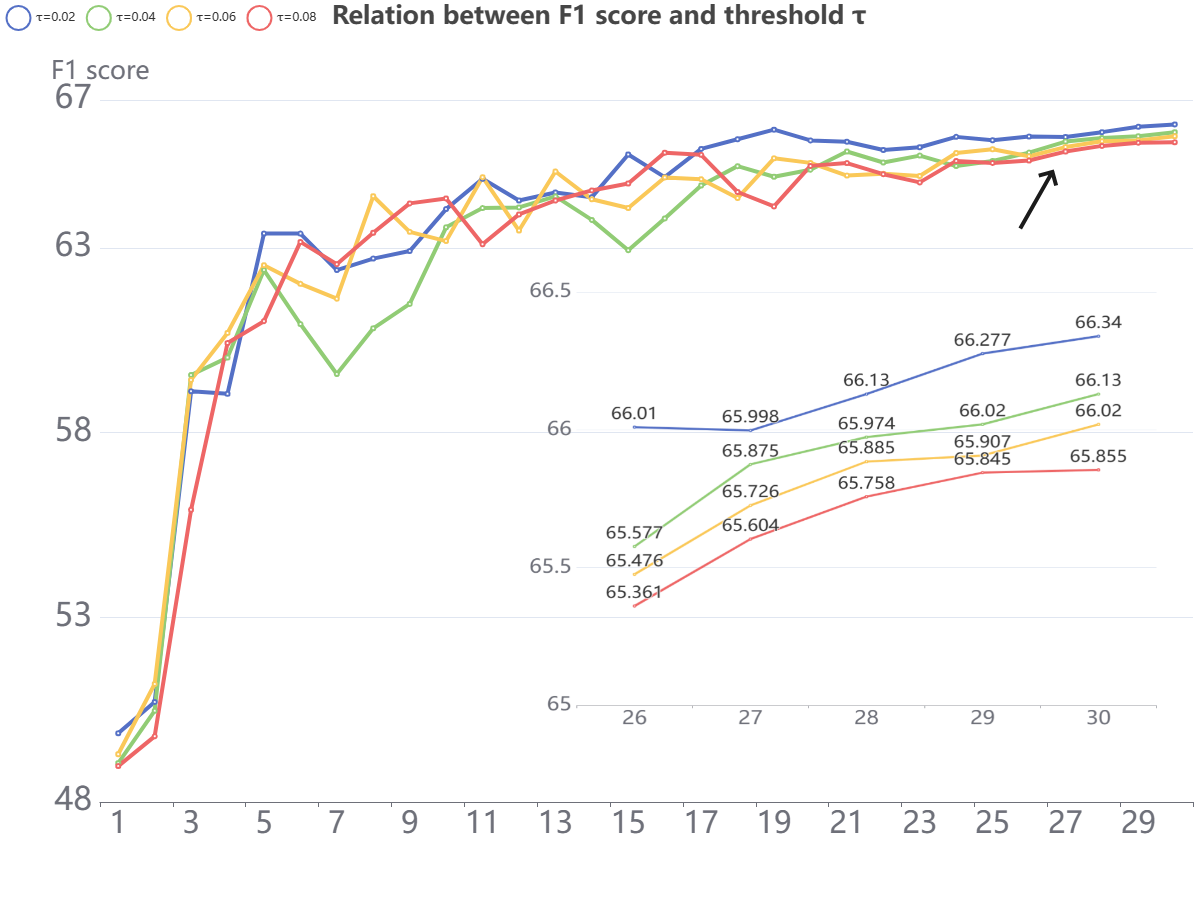
\includegraphics[width=4in]{./threshold.png}
\caption{Relation between $F_1$ score and threshold $\tau$ in the Co-occurrence relations construction.}
\label{fig.6}
\end{figure*}

Therefore, selecting an appropriate threshold is crucial for relation extraction tasks. It requires a delicate balance between noise and information loss to ensure that the generated relational graph is both accurate and interpretable. Our in-depth investigation into the influence of the threshold $\tau$ on noisy edges involved setting the threshold range to [0.02, 0.04, 0.06, 0.08]. Through repeatedly controlled experiments, it was consistently observed that, the $F_1$ score reached the highest value when the threshold $\tau$ is set to 0.04. As illustrated in one set of experimental results presented in Fig. \ref{fig.6}.


In order to show the co-occurrence between relations more clearly, we visualize some of the relations using conditional probabilities, as shown in Fig. \ref{fig.7}.  According to the Fig.\ref{fig.7}, we find that within the same co-occurrence relation, the probability of another relation differs depending on the preceding relation. For example, when the premise is relation "part of", p (applies to jurisdiction $\mid$ part of) = 0.32. However, when the premise relation is "applies to jurisdiction", p (part of $\mid$ applies to jurisdiction) = 0.65. The difference is due to the different number of co-occurrences of each relation with all others.

\begin{figure}[htbp]
\centering
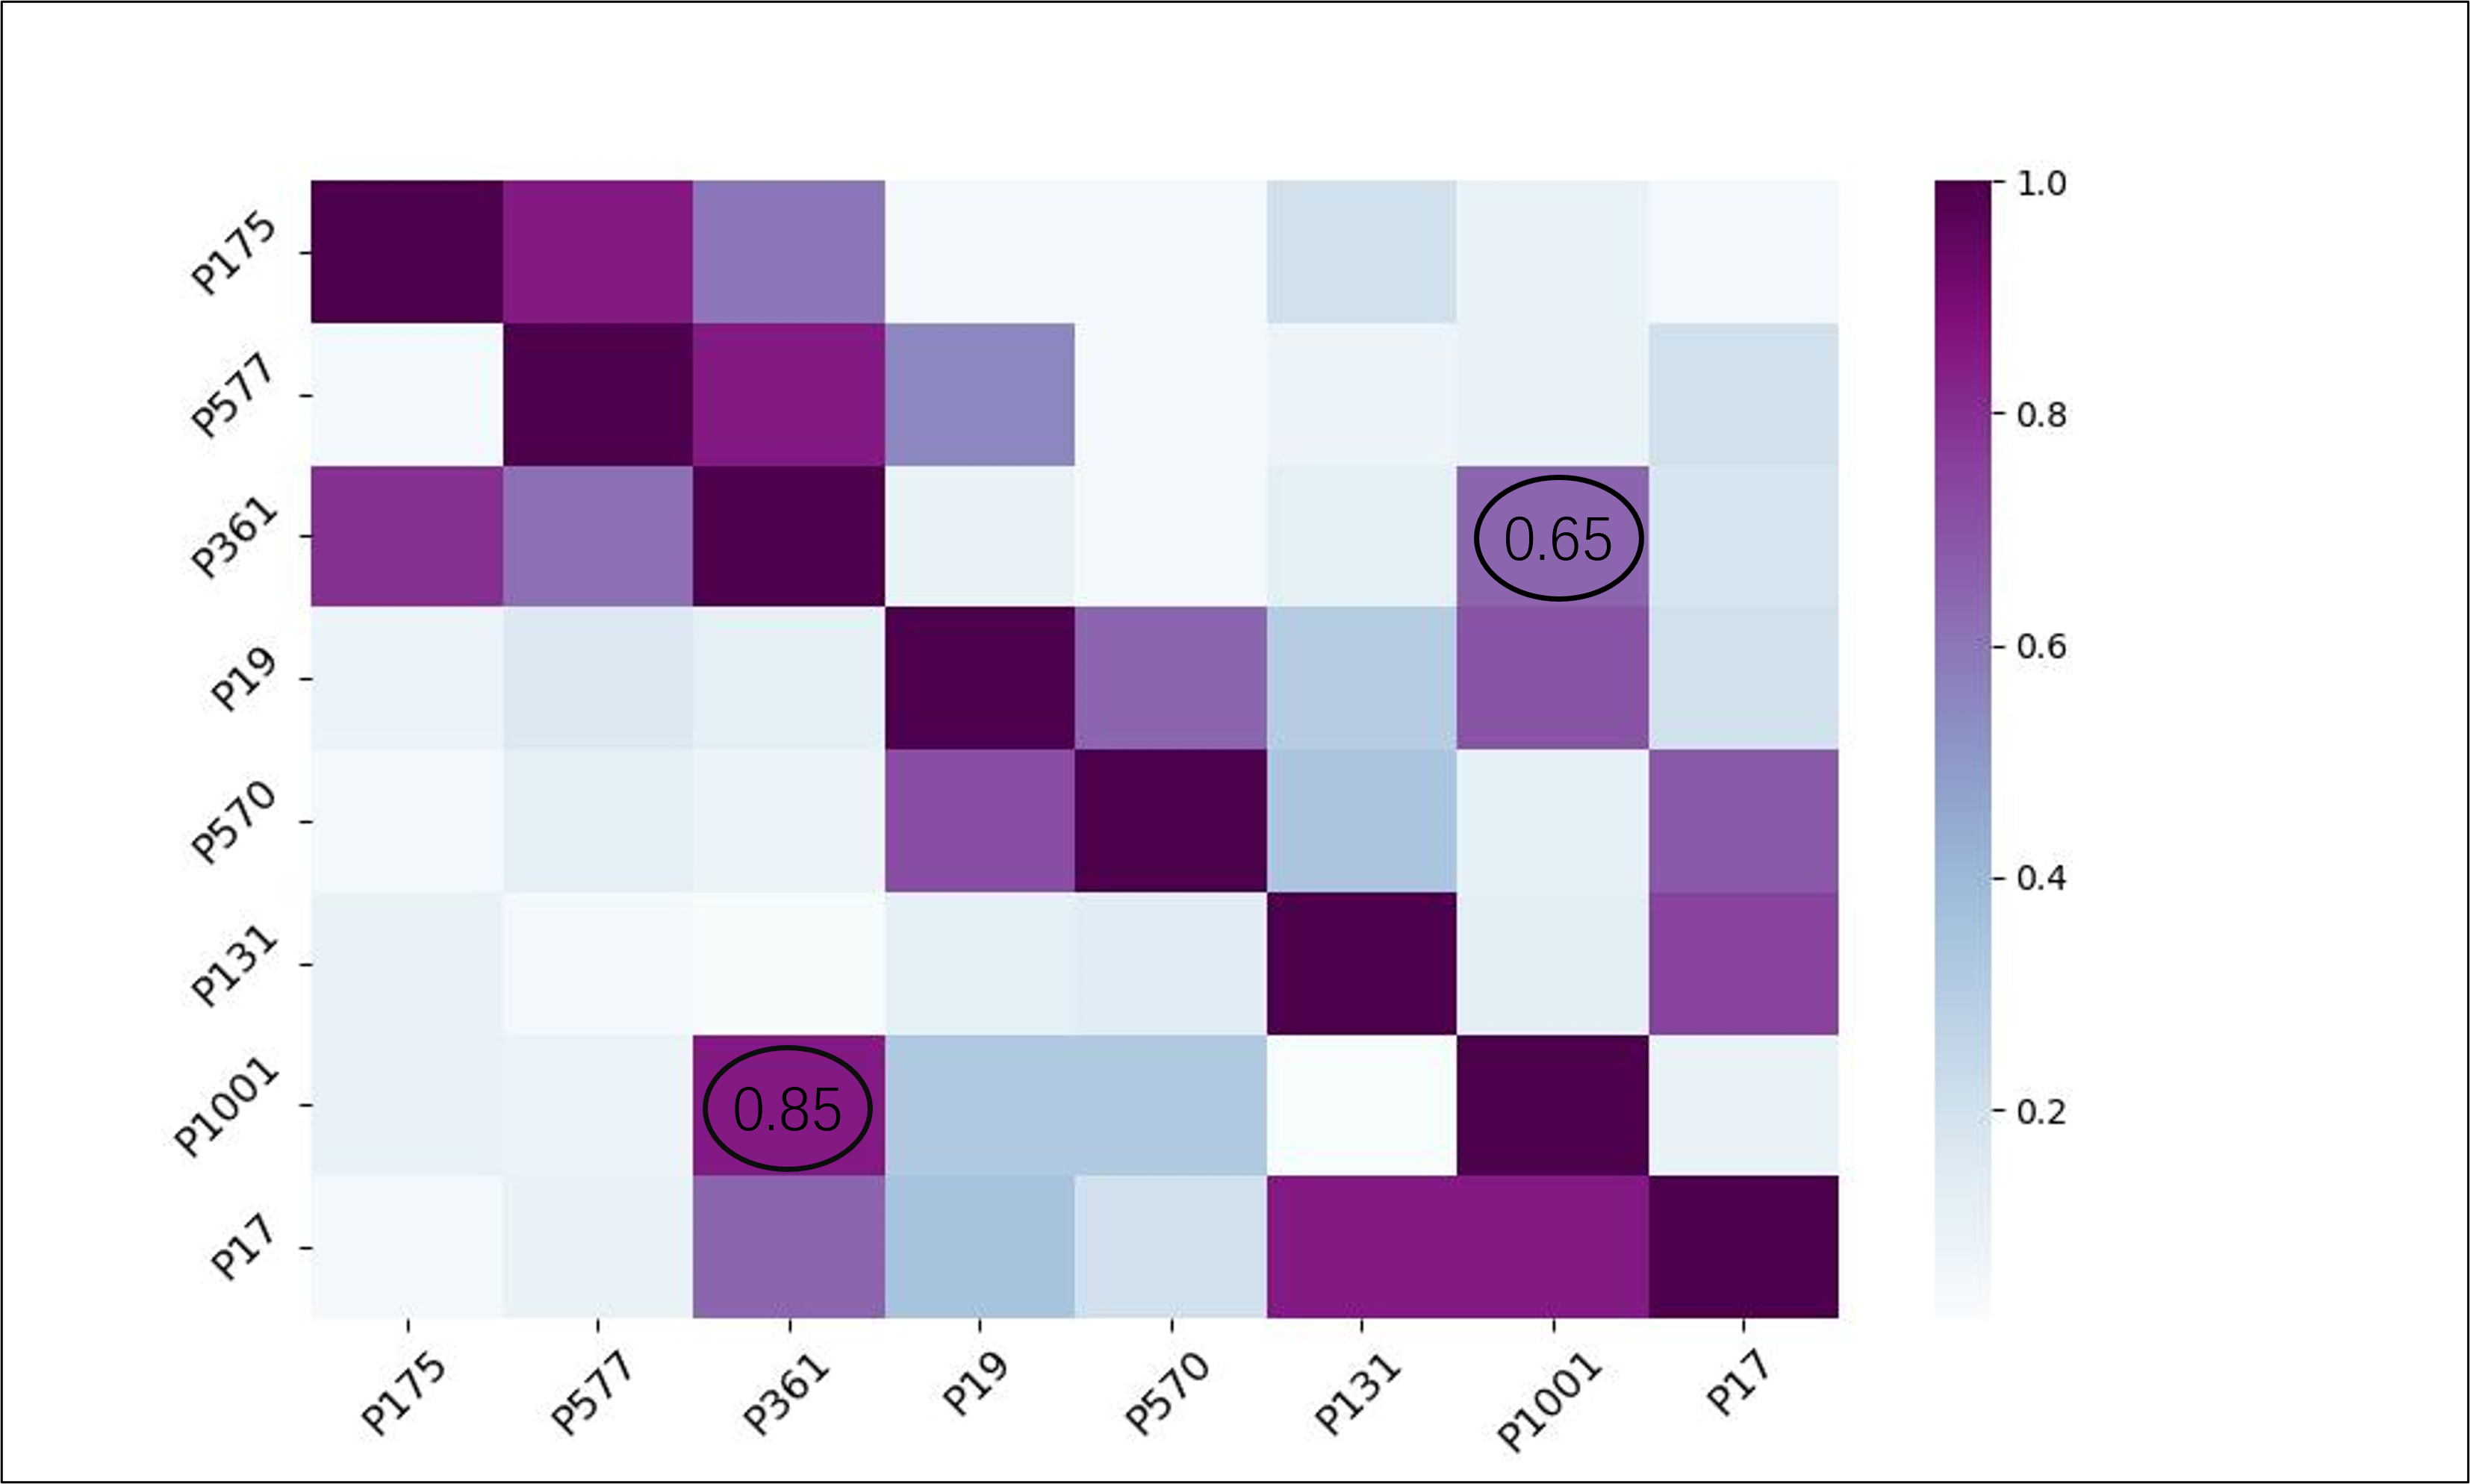
\includegraphics[width=3.5in]{./Co-relation.png}
\caption{Relation correlation heatmap. Refer to the Appendix for the relations represented by the axis numbers and the abscissa represents the precondition relation.}
\label{fig.7}
\end{figure}

\subsubsection{Analysis on The Number of BERT Layer}\label{subsubsec12}
BERT adopts a multi-layered Transformer structure, where each layer receives the output of the previous layer to form a cascade effect. The structure enables first few layers to focus more on the statement and local structure of the original input, while last few layers integrate semantic information passed down from the lower layers. 
\begin{table}[htbp]\centering
\caption{Effect of the number of BERT layers used on the $F_1$ score in PrLMs}\label{tab5}
\resizebox{8cm}{!}{%
\begin{tabular}{|l|c|}
\hline
{Number of BERT layers} &{Average $F_1$} \\
\hline
Last layer & 66.15 \\
\hline
Average of last three layers & 66.27 \\
\hline
\end{tabular}%
}
\end{table}

To be specific, at the BERT's last few layers, the self-attention mechanism primarily attends to the dependency relations between words in the input sequence, which makes the model to capture word-relative positions and local contextual information easily. As the number of layers increases, the model gradually could capture longer-distance dependency relations, allowing it to understand a more extensive context, which is crucial for learning semantic information.

In practical applications, we choose the value of the last layer and the average value of the last three layers to express the influence of the experimental results. In addition, we conduct five replicate experiments and take the average as the final result. The selection takes into account the contributions of features and semantic information at different levels in BERT, providing a more comprehensive and accurate representation of the model’s performance, the experimental results are shown in Table \ref{tab5}.



\subsection{Ablation analysis}\label{subsec4}
To investigate the roles of different modules in EG-ReCo, we conduct ablation study, and the results are presented in Table \ref{tab6}. We progressively remove parts related to RL-based evidence selection (Re -   RL) and Co-occurrence relations construction (Re - CO) from the complete EG-ReCo.

From the table, we observe that, when RL-based evidence selection or  Co-occurrence relations construction is removed, metric $lgn F_1,F_1$  and $Evi F_1$ have an obvious decrease in validation sets and test sets.  In addition, after removing RL-based evidence selection module, the score of $Evi F_1$  is 55.42 in the validation set and 55.63 in the test set, which decreases far more than removing Co-occurrence relations construction module. The situation is mainly due to the fact that, when RL-based evidence selection module is removed, the EG-ReCo may not be able to select more effective evidence sentences to predict the correct entity relation. However, the lack of Co-occurrence relations construction module may make the EG-ReCo unable to capture the potential association between entities, which affects the reasoning ability. These experiments show that, RL-based evidence selection module and Co-occurrence relations construction module play crucial roles in both relation prediction and evidence selection.

\begin{table*}[htbp]
\centering
\caption{Ablation study}\label{tab6}
\begin{tabular*}{\textwidth}{@{\extracolsep\fill}lcccccc}
\hline
Model & \multicolumn{3}{c}{Dev} & \multicolumn{3}{c}{Test} \\
& $lgn$ $F_1$ & $F_1$ & $Evi$ $F_1$ & $lgn$ $F_1$ & $F_1$ & $Evi$ $F_1$ \\
\hline
$\mathbf{EG-ReCo}$  & $\mathbf{64.51}$ & $\mathbf{66.34 }$ & $\mathbf{56.23}$ & $\mathbf{64.39 }$ & $\mathbf{66.56}$ & $\mathbf{56.69}$  \\
Re - RL & 63.94 & 66.01 & 55.42 & 64.07 & 66.13 & 55.63 \\
Re - Co & 63.87 & 65.94 & 55.97 & 63.81 & 65.91 & 56.31 \\
\hline
\end{tabular*}
\end{table*}


\section{Conclusion}\label{sec6}

In this paper, we propose a multiple and knowledge distillation DocRE method, named EG-ReCo. Firstly, we utilize human-annotated dataset to train a teacher model, and the trained teacher model adopt distantly-supervised dataset to obtain soft labels. Secondly, the soft labels are combined with distant supervision datasets to perform multiple self-training to obtain a student model. Furthermore, We adopt a human-annotated dataset to fine-tune the student model, which aims to make full use of the knowledge of the teacher model and improve the performance of the student model in order to compensate for the potential difference between the two datasets. Moreover, we design RL-based evidence selection module and Co-occurrence relations construction module to provide the accuracy of relation prediction and the ability of multi-relation extraction. Finally, extensive experiments results demonstrate that our method EG-ReCo can achieve the state-of-the-art performance.

In fields such as biology and medicine, biological entities have complex networks of interactions, such as the relations between proteins, genes, and diseases. Therefore, how to accurately capture and understand these complex relations is critical to driving drug discovery, building disease models, and revealing the mechanisms of cellular processes. Our proposed multi-relation extraction method can help researchers more comprehensively identify and analyze the interactions between these biological entities and their underlying mechanisms. However, we also notice that the performance of the proposed method degrades when dealing with extremely unbalanced long-tail relations. In the field of biology and medicine, the sample size of some important relations is very small, while the sample size of other irrelevant relations is relatively large. This long-tail distribution problem requires us to further optimize the evidence selection and relationship prediction strategies We plan to improve the model's ability to recognize low-frequency relations through fine-tuning strategies in RL modules or by using data enhancement techniques. Therefore, how to deal with long-tail class relations becomes the focus of our future work. 

\section*{Declarations}

Conflict of Interest: The authors declare no conflict of interest.

\section{Data Availability}
The data and resources utilized in this method are available as follows:

\begin{itemize}
    \item Code: The code used for our experiments is publicly accessible at \url{https://github.com/wanqiy/EG-ReCo}.
    \item Datasets: We utilized two publicly available datasets for our method:
    \begin{itemize}
        \item DocRED: Available at \url{https://github.com/thunlp/DocRED}.
        \item Re-DocRED: Available at \url{https://github.com/tonytan48/Re-DocRED}.
    \end{itemize}
    \item Test Results: The results on our test set are available online at \url{https://codalab.lisn.upsaclay.fr/competitions/365}.
\end{itemize}

\section*{Acknowledgments}
This work was financially supported by National Key R\&D Program of China(No.2020YFC2006602) , National Natural Science Foundation of China (No.62372318, No.62102278, No.62072324), Postgraduate Research \& Practice Innovation Program of Jiangsu Province(KYCX24\_3447).




%% The Appendices part is started with the command \appendix;
%% appendix sections are then done as normal sections


%% If you have bibdatabase file and want bibtex to generate the
%% bibitems, please use
%%
%%  \bibliographystyle{elsarticle-harv} 
%%  \bibliography{<your bibdatabase>}

%% else use the following coding to input the bibitems directly in the
%% TeX file.

% \begin{thebibliography}{00}

%% \bibitem[Author(year)]{label}
%% Text of bibliographic item






% \bibliographystyle{elsarticle-harv} 
% \bibitem[ ()]{}
\bibliography{ref.bib}

\appendix
\begin{table}[h]
\section{Partial relation sequence number}
%% \label{}
\caption{Partial relation sequence number}\label{app1}
\begin{tabular*}{\textwidth}{@{\extracolsep\fill}lcp{7cm}}
\toprule%
Wikidata ID & Name & Hypothesis Construction \\
\midrule
P17&	Country	&The sovereign state of this item sub. is obj.\\
P19	&Place of birth	The birth& location of the person, animal or fictional character sub. is obj\\
P131&	Located in the ATE	&Sub. is located on the territory of the following administrative entity obj\\
P175 &Performer&	The performer involved in the performance or the recoding of the work sub. is obj\\
P361&	Part of&	Obj. has part or parts sub.\\
P570&	Date of death&	The date on which sub. died is obj.\\
P577&	Publication date&	The data or point in time the work sub. is first published or released is obj.\\
P1001&	 Applies to jurisdiction&	The institution, law or public office sub. belongs to or has power over or applies to the country, state or municipality obj.\\
\hline
\end{tabular*}
\end{table}
% \end{thebibliography}
\end{document}

\endinput
%%
%% End of file `elsarticle-template-harv.tex'.
